 %\pdfoutput=1
\documentclass[conference]{IEEEtran}
\IEEEoverridecommandlockouts
% The preceding line is only needed to identify funding in the first footnote. If that is unneeded, please comment it out.
\usepackage[T1]{fontenc}
\usepackage{cite}
%\usepackage{caption}
%\usepackage{subcaption}
\usepackage{mathtools}
\usepackage{stackengine}
\def\delequal{\mathrel{\ensurestackMath{\stackon[1pt]{=}{\scriptstyle\Delta}}}}
\usepackage{amsmath,amssymb,amsfonts}
\usepackage{amsmath,epsfig,cite,amsfonts,amssymb,psfrag,subfigure}
\usepackage{graphicx}
\usepackage{blindtext}
\usepackage{textcomp}
\usepackage{xcolor}
\usepackage{algorithm}
\usepackage[noend]{algpseudocode}
\usepackage{amsthm}
\def\BibTeX{{\rm B\kern-.05em{\sc i\kern-.025em b}\kern-.08em
    T\kern-.1667em\lower.7ex\hbox{E}\kern-.125emX}}
\allowdisplaybreaks
\newtheorem{remark}{Remark}
\newtheorem{theorem}{Theorem}
\newtheorem{lemma}{Lemma}
\newtheorem{proposition}{Proposition}
\newtheorem{corollary}{Corollary}
\newcommand{\diag}{\mathop{\mathrm{diag}}}
\DeclareMathOperator{\E}{\mathbb{E}}
\usepackage[margin=0.7in]{geometry}
\usepackage[export]{adjustbox}
\DeclareMathOperator*{\argmax}{arg\,max}
\DeclareMathOperator*{\argmin}{arg\,min}
\setlength{\columnsep}{11mm}
\begin{document}

\title{Resource Allocation in an Open RAN System using Network Slicing\vspace{-.1cm}
}

\author{\IEEEauthorblockN{ Mojdeh Karbalaee Motalleb}
\IEEEauthorblockA{\textit{School of ECE} \\
\textit{Tehran University}\\
Tehran, Iran \\
mojdeh.karbalaee@ut.ac.ir}
\and
\IEEEauthorblockN{ Vahid Shah-Mansouri}
\IEEEauthorblockA{\textit{School of ECE} \\
\textit{Tehran University}\\
Tehran, Iran \\
vmansouri@ut.ac.ir}
\and
\IEEEauthorblockN{ Saeedeh Parsaeefard}
\IEEEauthorblockA{\textit{Department of ECE} \\
\textit{University of Toronto}\\
Toronto, Canada \\
saeede.parsaeefard@gmail.com}
}
%  \author{
%    \IEEEauthorblockN{Mojdeh Karbalaee Motalleb, Vahid Shah-mansouri}
%    \IEEEauthorblockA{School of ECE, College of Engineering, University of Tehran, Iran \\
%    Email: \{mojdeh.karbalaee, vmansouri\}@ut.ac.ir,
%    \vspace{-.2cm}
%  }


\maketitle

\begin{abstract}
Taking advantage of virtual Radio access network (v-RAN) and Cloud RAN (C-RAN), Open RAN (O-RAN) is introduced as the next generation of RAN systems. O-RAN leads to increased flexibility and openness and reduces operational costs, enabling new capabilities to be added to the network more quickly.
O-RAN separates RAN into three different units, namely Radio Unit (O-RU), Distributed Unit (O-DU), and Central Unit (O-CU).
In this paper, we study the problem of baseband resource allocation and virtual network function (VNF) activation in O-RAN architecture based on their service priority for different types of 5G services including enhanced mobile broadband (eMBB), ultra-reliable low latency communications (URLLC) and massive Machine Type Communications (mMTC) services.
Deploying network slicing, the isolation of different types of services in O-DU, O-CU, and user plane function (UPF) is performed.
The limited fronthaul capacity and the restriction of end-to-end delay are considered at the same time.
The optimization of baseband resources includes O-RU assignment, physical resource block (PRB), and power allocation. The main problem is a mixed-integer non-linear programming problem that is non-trivial to solve numerically.
Nevertheless, we break it down into two different steps where an iterative algorithm finds near optimal solution.
In the first step, we reformulate and simplify the problem to find the power allocation, PRB assignment, and the number of activated VNFs. In the second step, the O-RU association is achieved.
The proposed method is confirmed via simulation results which illustrate a higher achievable data rate than a baseline scheme that only optimizes one of the baseband resources and the FBDR algorithm described in the literature. Also, the simulation results demonstrate less end-to-end delay for the proposed method than the FBDR and baseline scheme.
   
\end{abstract}

\begin{IEEEkeywords}
Open Radio Access Network (O-RAN), Virtual Network Function (VNF), Network Slicing.
\end{IEEEkeywords}

\section{Introduction} 
One of the fifth-generation goals of the wireless cellular networks  is to achieve the desired QoS (such as rate, delay, power, ...) for different types of services. Network slicing is the best solution for this aim. A network slice is an end-to-end logical network that offers services with specific needs.  
Multiple isolated network slices run, manage, and work independently on the same infrastructure. 
Several implementations of network slicing include core slicing, RAN slicing, and slicing of both sections. 
Three types of services are introduced for 5th generation celluar networks, namely, enhanced mobile broadband (eMBB), ultra-reliable low latency communications (URLLC), and massive Machine Type Communications (mMTC) services. Each type of service requires a particular slice of network based on its QoS.
eMBB requires a higher transmission data rate in comparison with 4G systems. Moreover, eMBB service satisfies the demands of high capacity and throughout coverage.
URLLC requires low latency  and high reliability. URLLC contains services such as autonomous vehicles, tactile internet, or remote surgery.
mMTC consists of a vast number of low power internet of things (IoT) devices transmitting small payloads to a typical receiver. In addition, mMTC UEs include sensors for sensing, metering, and monitoring devices 
\cite{shen2020ai,setayesh2020joint,popovski20185g,dogra2020survey,kassab2018coexistence,alsenwi2021intelligent}.

Recently, RAN virtualization receives significant attention from industry and academia since it has remarkable benefits that increase flexibility and reduce CAPEX and OPEX and allow operators to add new capabilities to the network more quickly. In addition to RAN virtualization, openness and RAN intelligence are two pillars that encourage the Open Radio Access Network (O-RAN) Alliance to establish O-RAN as the next generation of RAN systems. 
The idea of O-RAN comes from the integration of virtual RAN (vRAN) and cloud RAN (CRAN), and it takes advantage of both. CRAN divides RAN into two parts, radio remote head (RRH) and baseband unit (BBU).  Several distributed RRHs can be connected to a centralized BBU,  called BBU-pool \cite{han2019research}. 
Unlike the previous generation of RAN that divides RAN into two parts, O-RAN separates RAN into three different units, namely Radio Unit (O-RU), Distributed Unit (O-DU), and Central Unit (O-CU). 
O-RU is a logical node that contains RF and lowers PHY. Moreover, the O-DU expresses another logical node that includes higher PHY, MAC, and RLC.
In addition, the O-CU contains two parts, which are the O-CU user plane (O-CU-UP) and O-CU control plane (O-CU-CP). O-CU-UP hosts PDCP-UP and SDAP, and O-CU-CP hosts PDCP-CP and RRC.
O-DU and O-CU are connected via open and well-defined interface $F_1$.
Moreover, O-DU is connected to a radio unit (O-RU) with an open fronthaul interface.
The architecture of O-RAN contains other principal logical nodes called Orchestration and Automation,
RAN Intelligent Controller (RIC)- Near Real-Time and O-Cloud. 
One of the necessities of the new generation of wireless networks is its intelligence.
Based on the requirement of an intelligent wireless network, O-RAN offers machine learning techniques. The two logical nodes RIC-Non Real-Time (which is placed in Orchestration and Automation node) and RIC- Near Real Time, implement the algorithms for network intelligence 
\cite{gavrilovska2020cloud,niknam2020intelligent,kazemifard2021minimum,both2021system,ORANArch,ORANML,lin2021toward}.

Network function virtualization (NFV) is referred to the separation of network software and hardware elements such that network function can run on commodity hardware. Virtual network functions (VNF) are system function blocks in NFV systems. This technology improves the system performance in the fifth generation of telecommunication networks. 
The key idea of the implementation of NFV is to decouple software from physical hardware, dynamic scaling, and the deployment of flexible network functions. The NFV technology offers to execute VNFs as virtual machines or containers on  cloud environment \cite{mijumbi2015network, luo2020online}.
As a result, some O-RAN components that include user plane function (UPF), O-CU, O-DU, and RAN Intelligent Controller (RIC)-near real-time, are virtualized and implemented as a VNF that can be run as virtual machines (VMs) or containers.
\subsection{Related Works}
The problem of resource allocation for network slicing in multi-tenant cellular networks has received attention recently \cite{feng2020dynamic,lee2018dynamic,lee2016new}.
In \cite{lee2018dynamic}, dynamic network slicing in multi-tenant heterogeneous CRAN (H-CRAN) is considered. The process of allocating network resources to users is discussed. The network slicing scheme includes a higher level and the lower level. The higher level manages user acceptance control, user communication that provides for radio unit association (RRH association to maximize user rates and allocate baseband resource capacity), the allocation of BBU capacity. Also, in the lower level, the allocation of power and physical resource blocks (PRB) is performed.
In \cite{xiang2020realization}, network slicing in the radio section is considered for fog RAN (F-RAN) system, in which, two network slices are set for hotspots and vehicle scenarios with related infrastructure. In \cite{elayoubi20195g,d2020toward}, the implementation of RAN level slicing is discussed in mobile network operator (MNO). Also, the problem of resource allocation is considered. Moreover, the paper faces the challenge of RAN slicing. The problem involves designing and managing multiple slices in the shared infrastructure efficiently while guaranteeing each slice's service level agreement (SLA).


Multiplexing eMBB and URLLC services on the same RAN and sharing the resources of these services is challenging, and many researchers pay attention to this issue.
In \cite{setayesh2020joint,yang2020should}, the problem of resource allocation in the coexistence of URLLC and eMBB services is considered based on their QoS. 
In \cite{alsenwi2021intelligent}, the problem of resource allocation for joint eMBB and URLLC services is formulated and solved by deep reinforcement learning.
 In \cite{saggese2021power}, the problem of power minimization for URLLC and eMBB services is presented for non-orthogonal multiple access (NOMA) and orthogonal multiple access (OMA).
 In \cite{korrai2020ran}, the authors proposed to allocate RAN resources for the network slicing system in coexistence of eMBB and URLLC services. The system guarantees the latency, the service rate, and the maintenance of reliability.

Virtualization technique for RAN and core is one of the exciting topics.  
In \cite{SystemCostMinimization,guo2016exploiting}, the authors solve the problem of obtaining beamforming and VMs activation in a C-RAN system with limited fronthaul capacity. 
This paper aims to minimize the energy cost with the system delay, fronthaul capacity, and rate constraint. 
Also, transmission and processing delay are modeled based on M/M/1 queuing theory to guarantee delay for the UEs.
 In \cite{luong2018joint,luong2018novel}, the problem of joint virtual computing resource allocation with beamforming is formulated; Also, the association of RRH to the UE is considered and solved using innovative methods.
In \cite{ali2019energy,ali2019energy1,ali2018joint}, the problem of joint power allocation and RRH association in the H-CRAN system is considered to maximize energy efficiency.
In \cite{amani2019power}, optimum power is obtained in massive MIMO aided C-RAN. Also the problem of RRH to BBU and the RRH to UE association is obtained. Moreover, the author talked about the feasible region to make the initial values possible.
\subsection{Main Contributions}
This study aims to optimize baseband resource allocation i.e., power allocation, PRB allocation, and O-RUs association, and VNF activation, to develop an isolated network slicing outline for different types of services in an O-RAN platform. In this paper, as depicted in Figure \ref{fig:c11}, the downlink of the ORAN system is studied. The main contributions of this paper are summarized as follow:
\begin{itemize}
\item This paper depicts a network slicing model for three different types of services introduced in 5G, i.e., eMBB, mMTC, and URLLC. The problem of radio resource allocation and VNF activation is studied in this paper in the O-RAN architecture.
We formulate the problem of baseband resource allocation to maximize the weighted throughput of the O-RAN system for a different types of services with specific QoS. 
\item The desired QoS conditions such as delay and throughput are considered for different types of services. We formulate the end-to-end mean delay of the system based on the number of activated VNFs and  user throughput.
We consider the limited fronthaul capacity and obtain the power and the capacity of each O-RU. We model the interference of neighboring O-RU and formulate the actual throughput
for different types of services. We also model the throughput of URLLC and mMTC based on their short packet transmission.
\item The main problem is mixed-integer non-linear programming that is extremely difficult to solve.
We perform a two-step iterative algorithm to solve it.
The two-step iterative algorithm is presented for the resource management framework with the first-step VNF activation, power allocation, PRB association, and the second-step O-RU association.
\item We reformulated and simplified the main problem for the first step to find an upper and lower bound for the number of activated VNFs and use lagrangian function and KKT conditions to find optimal power and PRB allocation.
For the second step, the problem of O-RU association can be converted to a multiple knapsack problem and solved by the Greedy algorithm.
\item We talk about the initial point and the feasible region for the numerical results and introduce a fast algorithm that is less complex than our method to realize the feasible region for our problem.
\end{itemize}  

\begin{figure*}
  \centering 
    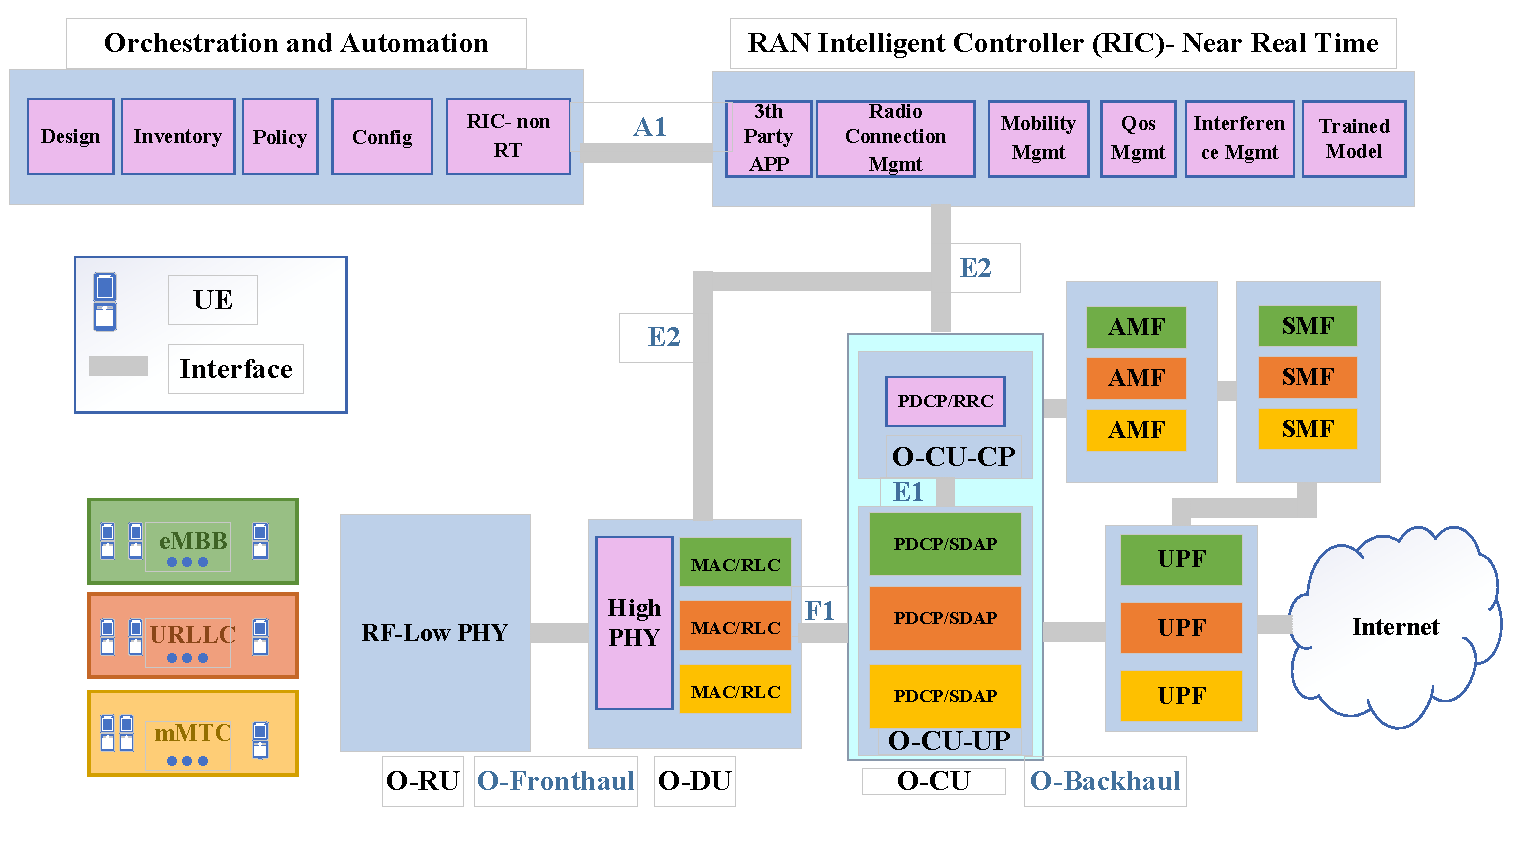
\includegraphics[scale = 0.7]{finalDraw.pdf}
    %\includegraphics[max height=30cm,max width=9.5cm]{Drawing15.eps}
    %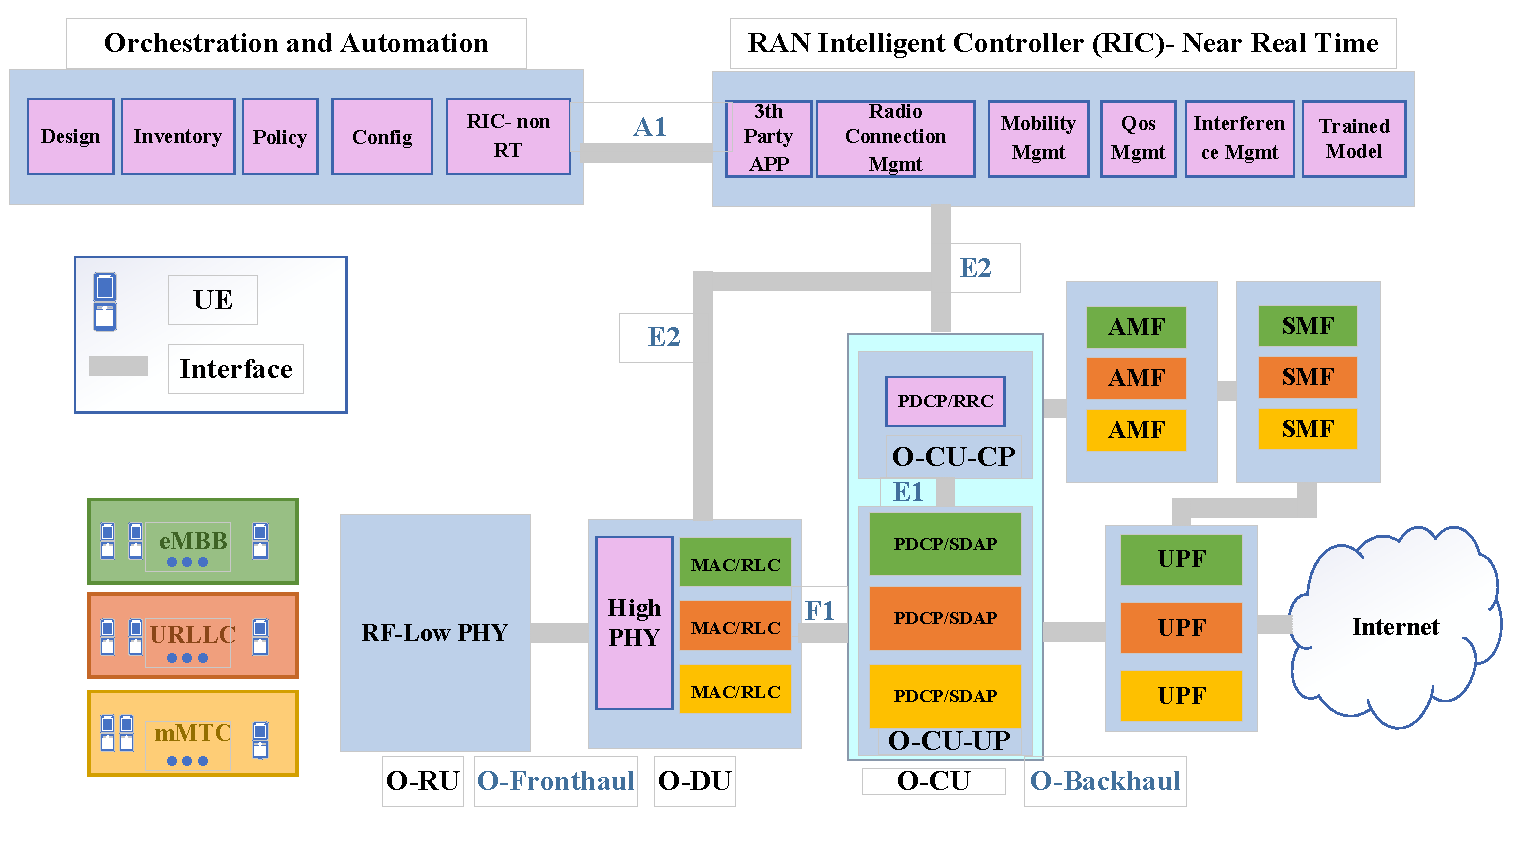
\includegraphics[width=\textwidth]{finalDraw.pdf}
  \caption{Network sliced ORAN system}
  \label{fig:c11}
\end{figure*}

The rest of this paper is organized as follows. The system model and the problem formulation are described in Section \ref{systemmodel}. The details of our proposed resource management algorithm are introduced in Section \ref{proAlg}. In Section \ref{NE}, numerical results are provided to evaluate the performance of the proposed algorithm. Section \ref{conc} concludes the  paper.

\section{System Model and Problem Formulation}\label{systemmodel}

In this section, we describe the downlink system in O-RAN with slicing as depicted in Figure \ref{fig:c11}. 
Firstly, we present the system model. Then, we obtain achievable data rates, power of O-RU, and the fronthaul capacity for the downlink (DL) of the ORAN system. Afterward, we discuss the mean delay and the power of VNFs.
Finally, the main problem is expressed.
\subsection{System Model}
There are three service types including mMTC, eMBB, and URLLC, which support different applications. There are $S_1$, $S_2$ and $S_3$ different applications for the mMTC, eMBB and URLLC service types, respectively and we have $S = S_1 + S_2 + S_3$. 
%{\color{red} explain pre-allocated more}
Therefore, there are $S$ pre-allocated slices serving these $S$ services;
Each pre-allocated slice contains reserved VNFs for the three logical nodes:
\begin{itemize}
\item The MAC/RLC functions in the O-DU logical node
\item The PDCP/SDAP functions in the O-CU-UP logical node
\item The UPF logical node
\end{itemize}

 There are $S_1$ slices for the first service type (eMBB), $S_2$ slices for the second service type (URLLC), and $S_3$ slices for the third service type (mMTC). So, each service request $s\in \{1,\ldots,S\}$ is served by its corresponding slice.

Each Service $s_j\in \{1,2,...,S_j\} $ consists of $U_{s_j}$ requests from  single-antenna UEs which require certain level of QoS. We notice that $j \in \{1,2,3\}$ indicates the service type.
There are different application requests which fall into one of these service categories. Each application request requires a specific QoS. Based on the application and QoS request, UE may be admitted and allocated to the resources.
Each slice $s_j \in \{1,2,...,S_j \}$, $j \in \{1,2,3\}$ consists of  $M_s^{d}$ VNFs for the processing of O-DU, $M_s^{c}$ VNFs for the processing of O-CU-UP and $M_s^{u}$ VNFs for the processing of UPF are required.

Assume we have $K$ physical resource blocks (PRBs) in this system.
All $K$ PRBs can be assigned to all UEs in each service.
Also, each VNF instance runs on a virtual machine (VM) that uses resources from the data centers.

In addition, there are $R$ multi-antenna O-RUs that are shared between slices. O-RU $r \in \{1,2,...,R \}$ has $J$ antennas for transmitting and receiving data. Also $\mathcal{R} = \{ r \ | \ r\in 1,2,...,R \}$ depicts the set of O-RUs. Moreover, all O-RUs have access to all PRBs.

%Coordinated multipoint (CoMP) system is considered here. 
\subsection{The Achievable Rate}
The SNR of the $i^{th}$ UE served at slice $s$ on PRB $k$ is obtained from
\begin{equation}\label{eq1}
\rho_{r,u(s,i)}^{k} =  \frac{|p_{r,u(s,i)}^{k}{\bold{h}_{r,u(s,i)}^{H \: k}} \bold{w}_{r,u(s,i)}^{k}|^2}{BN_0 + I_{r,u(s,i)}^{k}},
\end{equation} 
where $p_{r,u(s,i)}^{k}$ represents the transmission power from O-RU $r$ to the $i^{th}$ UE served at slice $s$ on PRB $k$. 
${\bold{h}_{r,u(s,i)}^{k}} \in \mathbb{C}^{J}$ is the vector of channel gain of a wireless link from 
$r^{th}$ O-RU to the $i^{th}$ UE in $s^{th}$ slice. In addition, $\bold{w}_{r,u(s,i)}^{k} \in \mathbb{C}^{J}$ depicts the  transmit beamforming vector from $r^{th}$ O-RU to the $i^{th}$ UE in $s^{th}$ slice that is the zero forcing beamforming vector to minimize the interference which is indicated as below
\begin{equation}
\bold{w}_{r,u(s,i)}^{k} = {\bold{h}_{r,u(s,i)}^{k}}({\bold{h}_{r,u(s,i)}^{H \: k}} {\bold{h}_{r,u(s,i)}^{k}})^{-1}
\end{equation}
Moreover, $g_{u(s,i)}^r \in \{0,1\}$ is the binary variable that illustrates whether O-RU $r$ served the $i^{th}$ UE that is allocated to $s^{th}$ slice or not. 
%Here, it is assumed that each UE is served by the nearest o-RU
Also, $BN_0$ denotes the power of Gaussian additive noise, and $I_{r,u(s,i)}^{k}$ is the power of interfering signals represented as follow
%{\color{red} use paranthesis in the following equation to clear +}
\begin{equation}\label{eqI}
\begin{split}
&I_{r,u(s,i)}^{k} =\\
 &\underbrace{\sum_{\substack{l=1 \\ l\neq i}}^{{U}_{s}} e^{k}_{u(s,i)}e^{k}_{u(s,l)}  p_{u(s,l)}^{k}\sum_{\substack{r'=1 \\ r'\neq r}}^{R}|{\bold{h}_{r',u(s,i)}^{H \: k}} \bold{w}_{r',u(s,l)}^{k} g_{u(s,l)}^{r'}|^2}_{\text{(intra-slice interference)}}+\\
&\underbrace{\sum_{\substack{n = 1 \\ n\neq s}}^{S}\sum_{l=1}^{{U}_s} e^{k}_{u(s,i)}e^{k}_{u(n,l)}  p_{u(n,l)}^{k}\sum_{\substack{r'=1 \\ r'\neq r}}^{R}|{\bold{h}_{r',u(s,i)}^{H \: k}} \bold{w}_{r',u(n,l)}^{k} g_{u(n,l)}^{r'}|^2}_{\text{(inter-slice interference)}}\\
&+\underbrace{  \sum_{j=1}^{{R}} {\sigma_q}^2 |\boldsymbol{h}_{r,{u(s,i)}}^k|^2 }_{\text{(quantization noise)}},
\end{split}
\end{equation}
%{\color{red} $\gamma_1$ is constant used instead of variable. }
%where $\gamma_{1} = e^{k}_{u(s,i)}e^{k}_{u(s,l)}$ and $\gamma_{2} = e^{k}_{u(s,i)}e^{k}_{u(n,l)}$.
where $e^{k}_{u(s,i)}$ is the binary variable to show whether the $k^{th}$ PRB is allocated to the UE $i$ in slice $s$, assigned to $r^{th}$ O-RU. %($\gamma_1$ and $\gamma_2$ are two variales. You  define on variable here.) 

To obtain SNR as formulated in \eqref{eq1}, let $y_{u(s,i)} $ be the received signal of UE $i$ in $s^{th}$ service formulated as
\begin{equation}\label{eq2}
y_{u(s,i)} = \sum_{r = 1}^{R}\sum_{k=1}^{K_s} \boldsymbol{h}^{H \: k}_{r,u(s,i)} g_{u(s,i)}^r e^k_{r,u(s,i)}\mathfrak{y}^k_{r,u(s,i)}+ z_{u(s,i)},
\end{equation}
%\boldsymbol{w}^k_{r,u(s,i)}p^k_{r,u(s,i)}
where $\mathfrak{y}^k_{r,u(s,i)} =\boldsymbol{w}^k_{r,u(s,i)}{p^{k \: \frac{1}{2}}_{r,u(s,i)}} x_{u(s,i)}+ \boldsymbol{q}_{r}$, $ x_{u(s,i)}$ depicts the transmitted symbol vector of UE $i$ in $s^{th}$ set of service,  $z_{u(s,i)}$ is the additive Gaussian noise $z_{u(s,i)} \backsim \mathcal{N}(0,N_0)$ and $N_0$ is the noise power.
In addition, $\boldsymbol{q}_{r} \in \mathbb{C}^{J }  $ indicates the quantization Gaussian noise 
($\boldsymbol{q}_{r} \backsim \mathcal{N}(0,{\sigma_q}^2\boldsymbol{I_{R}} )$), which is made from signal compression in O-DU.

The achievable data rate for the $i^{th}$ UE request in the $s_{1}^{th}$ application of service type 1 (eMBB) can be written as $\mathcal{R}_{u(s_1,i)}$ that is formulated as
\begin{equation}\label{eq3}
\begin{split}
\mathcal{{R}}_{r,u(s_1,i)}^{k} &=  B \log_2({1+ \rho_{r,u(s_1,i)}^{k}}) ,\\
\mathcal{R}_{u(s_1,i)}^{r} &= \sum_{k=1}^{K} B \log_2({1+ \rho_{r,u(s_1,i)}^{k}} e^k_{r,u(s_1,i)}),\\
\mathcal{R}_{u(s_1,i)} &= \sum_{r=1}^{R}\mathcal{R}_{u(s_1,i)}^{r} g^r_{u(s_1,i)},
\end{split}
\end{equation}
where $B$ is the bandwidth of system. 
$\mathcal{R}_{u(s_1,i)}^{r}$ is the achievable rate of RU $r$ to UE $i$ in slice $s_1$.
Since the blocklength in URLLC and mMTC is finite, the achievable data rate for the $i^{th}$ UE request in the $s_{j}^{th}$ ( $j \in \{2,3\}$) application of service type 2 (URLLC) and 3 (mMTC) is not achieved from Shannon Capacity formula. So, for the short packet transmission, the achievable data rate is approximated from following \cite{setayesh2020joint},
\begin{equation}\label{eq11}
\begin{split}
\mathcal{{R}}_{r,u(s_j,i)}^{k} &= B \log_2({1+ \rho_{r,u(s_j,i)}^{k}} - \zeta_{u(s_j,i)}^{k}){e}_{u(s_j,i)}^{k},\\
\mathcal{R}_{u(s_j,i)}^{r} &= \sum_{k=1}^{K} B (\log_2({1+ \rho_{u(s_2,i)}^{k}})- \zeta_{u(s_j,i)}^{k}){e}_{u(s_j,i)}^{k},\\
\mathcal{R}_{u(s_j,i)} &= \sum_{r=1}^{R}\mathcal{R}_{u(s_j,i)}^{r} g^r_{u(s_j,i)},
\end{split}
\end{equation}
where $j \in \{2,3\}$. Also we have %{\color{red} check paranthesis. }
\begin{equation}\label{shortPacket}
 \zeta_{u(s_j,i)}^{k} = \log_2({e})Q^{-1}(\epsilon) \sqrt{\frac{\mathfrak{C}_{u(s_j,i)}^{k}}{N_{u(s_j,i)}^{k}}},
\end{equation}
%{\color{red} what is transmission probability? }
where $\epsilon$ is the transmission error probability, $Q^{-1}$ is the inverse of Q function (i.e., Gaussian),
$\mathfrak{C}_{u(s_j,i)}^{k} = 1 - \frac{1}{(1+\rho_{u(s_j,i)}^{k})^2}$ depicts the channel dispersion of UE  $i$ at slice $s_j$, experiencing PRB $k$ and
$N_{u(s_j,i)}^{k}$ represents the blocklength of it. 
$\mathcal{R}_{u(s_j,i)}^{e,r}$ is the achievable data rate that is transmitted by O-RU $r$ to UE $i$ requesting service $s_j$.

If we replace $p_{u(s,l)}^{k}$ and $p_{u(n,l)}^{k}$ in \eqref{eqI} by $P_{s}^{max}$, an upper bound $\bar{I}_{r,u(s,i)}^{k}$ is obtained for $I_{r,u(s,i)}^{k}$. Therefore, $\bar{\mathcal{R}}_{u_{(s,i)}} \forall s , i$ is derived by using $\bar{I}_{r,u(s,i)}^{k}$ instead of $I_{r,u(s,i)}^{k}$ in  \eqref{eq11} and \eqref{eq3}.
\subsection{Power of the O-RU and the Fronthaul Capacity}
Let $P_r$ denote the power of the transmitted signal from the $r^{th}$ O-RU to all the UEs served by it. From \eqref{eq2}, the power of each O-RU $r$ is obtained as follows, 
%{\color{red} is this the sum rate of all users?}
\begin{equation}\label{pr}
P_r = \sum_{s=1}^{S}\sum_{k=1}^{K_s}\sum_{i=1}^{U_s}|\bold{w}_{r,u(s,i)}^{k}|^2 p_{r,u(s,i)}^{k} g_{u(s,i)}^r e^k_{r,u(s,i)}+ \sigma_{q}^2.
\end{equation}
Since we have a fiber link between O-RU and O-DU, the rate of users on the fronthual link between O-DU and the $r^{th}$ O-RU  is formulated as
%\cite{simeone2016cloud, 1111}
\begin{equation}\label{cr}
C_{r} = \log{\left(1+ \frac{\sum_{s=1}^{S}\sum_{k=1}^{K_s}\sum_{i=1}^{U_s}|\bold{w}_{r,u(s,i)}^{k}|^2 \mathcal{\alpha}^k_{r,u(s,i)} }{ \sigma_{q}^2}\right)},
\end{equation}
where $\mathcal{\alpha}^k_{r,u(s,i)}= p_{r,u(s,i)}^{k} g_{u(s,i)}^r e^k_{r,u(s,i)}$ and $\sigma_{q}^2$ is the power of quantization noise.
\subsection{Mean Delay}
In this part, the end-to-end mean delay for each service is obtained.
Suppose the mean total delay is depicted as $T_{\text{\text{tot}}}$,
\begin{equation}
\begin{split}
T^{\text{\text{tot}}} &=  T^{\text{proc}} + T^{tr} + T^{\text{pro}},\\
T^{\text{\text{proc}}} &=  T^{RU} + T^{DU} + T^{CU} + T^{UPF},\\
T^{tr} &= T^{fr,t} + T^{\text{mid},t} + T^{b,t},  \\
T^{\text{pro}} &= T^{fr,p} + T^{\text{mid},p} + T^{b,p}.  \\
\end{split}
\end{equation}
%{\color{red} I made a mistake and replaced pro with proc. Please correct them. Also, explain in more details the processing delay in this paragraph.}
%T_{\text{\text{tot}}} = T_{RU} + T_{front} + T_{DU} + T_{\text{mid}} + T_{CU} + T_{back} + T_{core} + T_{trans2net}
The total delay ($T^{\text{\text{tot}}}$), is the sum of the processing delay ($T^{\text{proc}}$), the transmission delay ($T^{tr}$), and the propagation delay ($T^{\text{pro}}$). 
The propagation delay is the time takes for a signal to reach its destination. It obtains based on the length of the fiber link and the capacity of the link ($T = L/c$, where $L$ is the length of the link and c is the capacity of the link). The total propagation delay ($T^{\text{pro}}$), is the sum of the propagation delay in the fronthaul link $T^{fr,p}$, the midhaul link $T^{\text{mid},p}$, and the backhaul link $T^{b,p}$.
Also, the transmission delay is the amount of time required to push all the packets into the fiber link.
Moreover, it can formulated as 
$T = \frac{\mathcal{\alpha}}{R}$, where $R$ is the sum-rate of the packet transmission in each link and $\mathcal{\alpha}$ is the mean arrival data rate of each link.
So the total transmission delay ($T^{tr}$) is the sum of the transmission delay in the fronthaul $T^{fr,t}$, the midhaul $T^{\text{mid},t}$, and the backhaul $T^{b,t}$.
In this paper, we focus only on the processing delays to find the optimal number of VNFs, and we ignore the other two delays for simplification;
So, we assume that the total delay is approximate to the processing delay.
%Here we assume the propagation delay and the transmission delay are negligible compared to the processing delay.
\begin{equation}
T^{\text{\text{tot}}} \approx T^{\text{proc}}
\end{equation}
\subsubsection{Processing Delay}
Assume the packet arrival of UEs follows a Poisson process with arrival rate $\lambda_{u(s,i)}$ for the $i^{th}$ UE of the $s^{th}$ service (or slice).
Therefore, the mean arrival data rate of the $s^{th}$ slice in the UPF layer is $\alpha_{s}^U = \sum_{u=1}^{U_s}\lambda_{u(s,i)}$.
Assume the mean arrival data rate of the UPF layer for slice $s$ ($\alpha_{s}^U$) is approximately equal to the mean arrival data rate of the O-CU-UP layer ($\alpha_{s}^C$) and the O-DU ($\alpha_{s}^D$). so $\alpha_{s} =\alpha_{s}^U \approx \alpha_{s}^C \approx \alpha_{s}^D$,
Because the amount of data traffic transferred along the route (regardless of frame changes) is constant.
Since, by using Burke’s theorem, the mean arrival data rate of the second and third layers, which are processed in the first layer, is still poisson with rate $\alpha_{s}$.
It is assumed that there are load balancers in each layer for each service to divide the incoming traffic to VNFs equally. %\cite{frdl,luong2018novel,luong2018novel1}.
Suppose the baseband processing of each VNF is depicted as M/M/1 processing queue.
Each packet is processed by one of the VNFs of a slice. So, the mean delay for the $s^{th}$ slice in the O-DU, the O-CU, and the UPF is modeled as M/M/1 queue, is formulated as follows, respectively \cite{SystemCostMinimization,luong2018joint,luong2018novel},
\begin{equation}
\begin{split}
T_{s}^{DU} &= \frac{1}{\mu_s^d - \alpha_{s}/{M_s^{d}}},\\
T_{s}^{CU} &= \frac{1}{\mu_s^c - \alpha_{s}/{M_s^{c}}},\\
T_{s}^{UPF} &= \frac{1}{\mu_s^u - \alpha_{s}/{M_s^{u}}},\\
\end{split}
\end{equation}
where $M_s^{d}$, $M_s^{c}$ and 
$M_s^{u}$ are the variables that depict the number of VNFs in O-DU, O-CU-UP and UPF, respectively. 
Moreover, $1/\mu_s^d$, $1/\mu_s^c$, and $1/\mu_s^u$ are the mean service time of the O-DU, O-CU, and the UPF layers, respectively.
Besides, $\alpha_{s}$ is the  arrival rate which is divided
by load balancer before arriving to the VNFs. The arrival rate of each VNF in each layer for each slice 
$s$ is $\alpha_{s}/{M_s^{i}}$ $ i \in \{d,c, u\}$.

$T_{u(s,i)}^{RU}$ is the mean transmission delay of the $i^{th}$ UE of the $s^{th}$ service on the wireless link.
 The arrival data rate of wireless link for each UE $i$ of service $s$ is $\lambda_{u(s,i)}$
As a result, we have $\sum_{i = 1}^{U_s} \lambda_{u(s,i)} = \alpha_s$.
Moreover, The service time of transmission queue for UE $i$ requesting service $s$ has
an exponential distribution with mean $1/R_{u(s,i)}$ and can be modeled as a M/M/1 queue \cite{SystemCostMinimization,luong2018joint,luong2018novel}.
 
Therefore, the mean delay of the transmission layer for UE $i$ in slice $s$ is
\begin{equation}
 T_{u(s,i)}^{RU} = \frac{1}{R_{u(s,i)} - \lambda_{u(s,i)}}.
\end{equation}

So, the mean processing delay for UE $i$ in slice $s$ is 
\begin{equation}
T^{\text{proc}}_{u(s,i)} =  T^{RU}_{u(s,i)} + T^{DU}_{s} + T^{CU}_{s} + T^{UPF}_{s}.
\end{equation}
Hence, for the simplification and focusing on the processing delay, we assume $T^{\text{\text{tot}}}_{u(s,i)} \approx T^{\text{proc}}_{u(s,i)} $. %{\color{red} what results in this approximation?}
%Furthermore, the mean arrival data rate of the each link ($\textstyle \alpha_{s}^i$ , $i \in \{RU,DU,CU,UPF\}$) is approximately equal to others ($\textstyle \alpha_{s} \approx \alpha_{s}^i$ , $i \in \{RU,DU,CU,UPF\}$).  
\subsection{VNF Power}
%{\color{red} Assume the power consumption of the baseband processing, the VNFs cost of a slice $s$ is depicted as $\phi_{s}$. Sentence has no meaning.} 
Assume the power consumption of each VNF in each logical node (the O-DU, the O-CU, and the UPF) in the slice s, is depicted as $\phi_{s}^d$, $\phi_{s}^c$, and $\phi_{s}^u$, respectively. 

So the system's total cost of energy of all the slices can be represented as
\begin{equation*}
\textstyle \phi_{\text{\text{tot}}} = \sum_{s=1}^{S}\phi_{s},
\end{equation*}
where $\phi_{s}$ is obtained from
\begin{equation}
\phi_{s} = M_s^u \phi_s^u + M_s^c \phi_s^c+ M_s^d \phi_s^d.
\end{equation}
Moreover, $\phi_s^u$, $\phi_s^c$, and $\phi_s^d$ are the fixed cost of energy in UPF, O-CU, and O-DU, respectively. 
\subsection{Problem Statement}
Suppose slice $s$ (which is assigned to service s) has the priority factor $\delta_s$ where $\sum_{s=1}^S \delta_s =1$.
The priority factor of each slice is obtained according to the service level agreement (SLA) of that service to have a fairness in the system. 
%{\color{red} explain why you introduce priority factor.}
This paper aims to maximize the sum-rate of all UEs with the presence of constraints as follows. %{\color{red} where did you define the objective? what is R bar?}
\begin{subequations}\label{problem}
\begin{alignat}{4}
\max\limits_{\boldsymbol{P}, \boldsymbol{E}, \boldsymbol{M}, \boldsymbol{G} }   \quad &  \sum_{s=1}^{S}\sum_{i=1}^{U_s}\delta_s \bar{\mathcal{R}}_{u_{(s,i)}} \ \\
\text{subject to} \quad  &  P_r \leq P^{max}_{r} \quad \forall r
 \label{c11} \\
&p_{r,u(s,i)}^{k}  \geq 0  \quad \forall i,\forall r,\forall s, \forall k,\label{c12} \\
&p_{r,u(s,i)}^{k}  \leq P_{s}^{max}  \quad \forall i,\forall r,\forall s, \forall k,\label{c12-1} \\
&\bar{\mathcal{R}}_{u_{(s,i)}} \geq \mathcal{R}_{{s}}^{min} \quad \forall s, \label{c13} \\
%&\mathcal{R}_{u_{(s_2,i)}}^u \geq  \mathcal{R}_{min}^{s_2,u} \quad \forall s_2, \label{c14} \\
& C_r \leq C^{max}_r \quad \forall r, \label{c15}\\ 
&T^{\text{\text{tot}}}_{u(s,i)}  \leq T^{max}_{s} \quad \forall i,\forall s,\label{c16} \\
& \mu_s \geq \alpha_s/M_s \quad \forall s,\label{c16-1} \\
& \bar{\mathcal{R}}_{u_{(s,i)}} \geq {\lambda}_{u_{(s,i)}} \quad \forall i,\forall s,\label{c16-2} \\
& 0 \leq M_s \leq M^{max}_s  \quad \forall s,\label{c16-3}\\
%& P_r\{E_1, E_2, E_3, E_4\} \leq \epsilon_s \quad \forall s_2, \label{c166}\\
& \sum_{r}g^r_{u(s,i)} = 1  \quad \forall s,\forall i, \label{c17}  \\
& \sum_{k =1}^{K_s} g^r_{u(s,i)} e^{k}_{r,u(s,i)} \geq 1  \quad \forall s,\forall i ,\forall r \label{c18-1} \\
& \sum_{s =1}^{S}\sum_{i=1}^{U_s}g^r_{u(s,i)} e^{k}_{r,u(s,i)} \leq 1  \quad \forall s,\forall i ,\forall r \label{c18} \\
& \phi^{\text{\text{tot}}}  \leq \phi^{max}, \label{c19} \\
& g^r_{u(s,i)} \in \{0,1\} \quad \forall s,\forall i, \label{c20}  \\
& e^k_{r,u(s,i)} \in \{0,1\} \quad \forall s,\forall i, \label{c21}  
\end{alignat}
\label{constraints}
\end{subequations}
\noindent where $\bar{\mathcal{R}}_{u_{(s,i)}}, \:\:\forall s , \forall i$ is derived by using $\bar{I}_{r,u(s,i)}^{k}$ instead of $I_{r,u(s,i)}^{k}$ in  \eqref{eq11} and \eqref{eq3}.
In addition, $\boldsymbol{P} =[p_{r,u(s,i)}^{k}], \:\: \forall s , \forall i, \forall r, \forall k $, is the matrix of power for UEs, $\boldsymbol{E} =[e_{r,u(s,i)}^k], \:\: \forall s , \forall i, \forall r, \forall k$ indicate the binary variable for PRB association. Moreover, $\boldsymbol{G} =[g_{u(s,i)}^r], \:\: \forall s , \forall i, \forall r$ is a binary variable for O-RU association. Furthermore, $M = [M_s^d, M_s^c, M_s^u], \:\: \forall s$ is the matrix that shows the number of VNFs in each layer of slice.
\eqref{c11}, \eqref{c12} and \eqref{c12-1} indicate that the power of each O-RU does not exceed the maximum power, the power of each UE is a positive integer value, and the power of each UE in each service does not exceed the maximum power of each service, respectively.  
Also, \eqref{c13} shows that the rate of each UE requesting each type of service, i.e., eMBB, mMTC, and URLLC, is more than a threshold, respectively.
\eqref{c15} and \eqref{c16} expressed the limited fronthaul capacity and the limited end-to-end delay of the received signal, respectively.
\eqref{c16-1} and \eqref{c16-2} denoted the stability of the M/M/1 queue model.
\eqref{c16-3} restricted the number of VNF in each slice due to the limited resources.
%\eqref{c16} is a reliability condition that the delay in each layer should be less than the threshold.
\eqref{c17} and \eqref{c18-1} guarantee that O-RU and PRB are associated with the UE, respectively.
Also, \eqref{c18} ensures that each PRB can not be assigned to more than one UE associated with the same O-RU.
In addition, \eqref{c19} indicates that the fixed cost of energy of VNFs in each slice does not exceed the threshold. 
Moreover, \eqref{c20} and \eqref{c21} depict that $\boldsymbol{E}$ and $\boldsymbol{G}$ are matrix of binary variables.
\section{Proposed Algorithm}\label{proAlg}
In this section, we first apply some simplifications to the system; Solving the problem \eqref{problem} is complicated since this is non-convex mixed-integer non-linear problem (MINLP) with a binary variable and an integer variable. 
We applied some simplifications and use an iterative heuristic algorithm to solve the problem.
We solve this problem in two levels, iteratively, until it converges \cite{ali2018joint}.

In the first level, the main purpose is to allocate adequate PRBs and the power to the UEs and allocate enough activated VNFs
to each slice. So, at this level, we would like to obtain the variables $\boldsymbol{P}, \boldsymbol{E},$ and $\boldsymbol{M}$.
Despite the simplification of the problem
\eqref{problem}, it is still NP-hard and challenging to solve. Therefore,
we relax the variable $\boldsymbol{E}$ \cite{lee2018dynamic,ali2018joint} and reformulating the constraint \eqref{c16},
to turn them into a jointly-convex problem; Afterward, we solve this problem using a conventional dual Lagrangian method. 
In the second level, finding the optimal O-RU association, $ \boldsymbol{G}$, is concerned with the fixed parameter of power, PRB allocation, and the number of activated VNFs.   
We repeat this procedure until the algorithm converges.

\subsection{Sub-Problem 1}\label{sub1}
Suppose that $\boldsymbol{G}$ is fixed, we want to obtain $\boldsymbol{P}, \boldsymbol{E}$ and $\boldsymbol{M}$.
Here, we first simplify and relax the parameters to convexify the problem.

As we mentioned before, by replacing $p_{u(s,l)}^{k}$ and $p_{u(n,l)}^{k}$ in \eqref{eqI} with $P^{max}_s$, an upper bound $\bar{I}_{r,u(s,i)}^{k}$ is obtained for $I_{r,u(s,i)}^{k}$, and also the lower bound $\bar{\rho}_{u(s,i)}^{k}$ is achieved
for $\rho_{u(s,i)}^{k}$. 
Moreover, the lower bound $\bar{\mathcal{R}}_{u_{(s,i)}}, \forall s , \forall i$ for  ${\mathcal{R}}_{u_{(s,i)}}$ is obtained by replacing $I_{r,u(s,i)}^{k}$ with $\bar{I}_{r,u(s,i)}^{k}$ in \eqref{eq11} and \eqref{eq3} and make these equations become concave functions.

Suppose $\hat{\rho}_{r,u(s,i)}^{k} =  \frac{|P_{s}^{max}{\bold{h}_{r,u(s,i)}^{H \: k}} \bold{w}_{r,u(s,i)}^{k} g_{u(s,i)}^r|^2}{BN_0}$. 
we replace ${\rho}_{r,u(s,i)}^{k}$ with $\hat{\rho}_{r,u(s,i)}^{k}$ in \eqref{shortPacket}, to convexify the \eqref{eq11} for the URLLC and mMTC services that have the short packet transmission.
So, a lower bound for \eqref{eq11} is given that is a concave function.
\begin{equation}
\begin{split}
\bar{\mathcal{R}}_{u(s_j,i)}^{r} &= \sum_{k=1}^{K_{s_j}} B (\log_2({1+ \bar{\rho}_{u(s_2,i)}^{k}})- \hat{\zeta}_{u(s_j,i)}^{k}){e}_{u(s_j,i)}^{k}\\
\bar{\mathcal{R}}_{u(s_j,i)} &= \sum_{r=1}^{R}\bar{\mathcal{R}}_{u(s_j,i)}^{r}\\ 
 \hat{\zeta}_{u(s_j,i)}^{k} =& log_2({e})Q^{-1}(\epsilon) \sqrt{\frac{\hat{\mathfrak{C}}_{u(s_j,i)}^{k}}{N_{u(s_j,i)}^{k}}})\\
 \hat{\mathfrak{C}}_{u(s_j,i)}^{k} =& 1 - \frac{1}{(1+\hat{\rho}_{u(s_j,i)}^{k})^2}\\
\end{split}
\end{equation}
Without loss of generality, assume that UPF, O-CU and O-DU use the processors with the same processing capability. We notice that it makes the formulation simpler. However, loosing this assumption does not change the formulation significantly and the problem can be solved in the same manner. Therefore, we have $\mu_s = \mu_s^u \approx \mu_s^c \approx \mu_s^d $. Moreover, as mentioned before,
the mean arrival data rate of the UPF layer for a service $s$ ($\alpha_{s}^U$) is equal to the mean arrival data rate of the O-CU-UP layer ($\alpha_{s}^C$) and O-DU ($\alpha_{s}^D$). So $\alpha_{s} =\alpha_{s}^U \approx \alpha_{s}^C \approx \alpha_{s}^D$. Again, this assumption only simplifies the notations and loosing it does not make the solution inefficient.
These assumptions lead to having the same processing power for each layer $\phi_s^u = \phi_s^c =\phi_s^d $.
As a result, we have $M_s = M_s^u = M_s^c = M_s^d $.
Using the above assumption, we have $T^{DU}_{s} = T^{CU}_{s} = T^{UPF}_{s}$ and 
\begin{equation}
\begin{split}
T^{\text{proc}}_{s} &=  T^{RU}_{s} + T^{DU}_{s} + T^{CU}_{s} + T^{UPF}_{s} \\
                     &=  T^{RU}_{s} + 3\times T^{DU}_{s}.
\end{split}
\end{equation}
In the following, we define a lemma to find the upper and lower bound for the optimal number of VNFs based on the achievable rates. Afterward, we obtain the formula to attain the optimal number of VNFs.  
\begin{lemma}
The optimal number of VNFs in each slice s can be achieved by the 
$M_s = \max\{\mathtt{M}_{u(s,i)} | i \in 1,2,..., U_s\} \quad \forall s$.
where, $\mathtt{M}_{u(s,i)} = \frac{\alpha_s(T^{max}_s R_{u(s,i)}-T^{max}_s\lambda_{u(s,i)} -1)}{(T^{max}_s\mu_s-3)(R_{u(s,i)}-\lambda_{u(s,i)}) - \mu_s }$ for each UE $i$ in slice $s$.

\end{lemma}
%{\color{red} add one sentence before lemma to motivate why you need this lemma. The whole part is a lemma? It is too long. Where is the proof?}
\begin{proof}
In problem \eqref{problem}, the constraint \eqref{c16} can be reformulated as
$ \forall i,\forall s$
\begin{equation}
\begin{split}
&T^{\max}_s \geq\frac{1}{R_{u(s,i)} - \lambda_{u(s,i)}} + \frac{3}{\mu_s - \alpha_{s}/{M_s}}  \\
&M_s \geq \frac{\alpha_s(T^{\max}_s R_{u(s,i)}-T^{\max}_s\lambda_{u(s,i)} -1)}{(T^{\max}_s\mu_s-3)(R_{u(s,i)}-\lambda_{u(s,i)}) - \mu_s }\\
\end{split}
\end{equation}
Also from equations in \eqref{c19}, \eqref{c16-1} and \eqref{c16-3}, we have
\begin{equation}
\alpha_s/\mu_s\leq M_s \leq \min\{M^{\max}, \phi_{\max}/{3\phi_s}\}
\end{equation}
We denote $ \mathfrak{M}_s= \min\{M^{max}, \phi_{max}/{3\phi_s}\}$.
Thus, if we restrict constraint \eqref{c16} to equality, constraint \eqref{c16} is still valid.
Also, we have the following inequality.
\begin{equation}\label{eqDelay}
\alpha_s/\mu_s\leq \frac{\alpha_s(T^{max}_s R_{u(s,i)}-T^{max}_s\lambda_{u(s,i)} -1)}{(T^{max}_s\mu_s-3)(R_{u(s,i)}-\lambda_{u(s,i)}) - \mu_s } \leq \mathfrak{M}_s
\end{equation}
In equation \eqref{eqDelay}, $0\leq \frac{\alpha_s(T^{max}_s R_{u(s,i)}-T^{max}_s\lambda_{u(s,i)} -1)}{(T^{max}_s\mu_s-3)(R_{u(s,i)}-\lambda_{u(s,i)}) - \mu_s }$ is established due to the fact that 
the numerator and the denominator will both have the same sign.
In the numerator, according to the \eqref{c16-2}, $ R_{u(s,i)}-\lambda_{u(s,i)} \geq 0$, and as we know that $\alpha_s \geq 0$, we have $ \alpha_s (R_{u(s,i)}-\lambda_{u(s,i)}) \geq 0 $.
If we assume that the $(R_{u(s,i)}-\lambda_{u(s,i)})T^{max}_s \geq 1$, the numerator will be positive.
$(R_{u(s,i)}-\lambda_{u(s,i)})T^{max}_s \geq 1$ since the order of $T^{max}_s$ is about milli second and the difference between achievable rate and packet rate can be more than $1/T^{max}_s$.
Therefore, to ensure that this constraint will be valid, we restrict constraint \eqref{c16-2} to $R_{u(s,i)} \geq \lambda_{u(s,i)} + 1/T^{max}_s$.
So the numerator will be positive.
In the denominator, we can say that $(T^{max}_s\mu_s)(R_{u(s,i)}-\lambda_{u(s,i)}) - \mu_s \geq 0 $, since,  
$\mu_s \geq 0$ and
$(R_{u(s,i)}-\lambda_{u(s,i)}) \geq 1/T^{max}_s$ as mentioned above.
%Therefore, we need to have the constraint below.
%\begin{equation}\label{constraint16}
%\alpha_s/\mu_s\leq \frac{\alpha_s(T^{max}_s R_{u(s,i)}-T^{max}_s\lambda_{u(s,i)} -1)}{(T^{max}_s\mu_s-3)(R_{u(s,i)}-\lambda_{u(s,i)}) - \mu_s } \leq \mathfrak{M}_s
%\end{equation}

The left side of the equation \eqref{eqDelay}, leads to $R_{u(s,i)} \geq \lambda_{u(s,i)}$ that is the constraint \eqref{c16-2}. 
For the right side, by reformulating the equation \eqref{eqDelay}, we have a new constraint $\forall i, \forall s$ as below,
%\begin{equation}\label{RM}
%\begin{split}
%\mathcal{R}_{u(s,i)} &\geq \frac{\mathfrak{M}_s \mathit{\langle}_{u(s,i)} - \alpha_s(T^{max}_s\lambda_{u(s,i)} +1) }{\mathfrak{M}_s (T^{max}_s\mu_s-3)-\alpha_s T^{max}_s},\\
% \mathit{\langle}_{u(s,i)}&=(T^{max}_s\mu_s-3)\lambda_{u(s,i)} + \mu_s,\\
%\varpi_{u(s,i)} &= \frac{\mathfrak{M}_s \mathit{\langle}_{u(s,i)} - \alpha_s(T^{max}_s\lambda_{u(s,i)} +1) }{\mathfrak{M}_s (T^{max}_s\mu_s-3)-\alpha_s T^{max}_s},\\
%\mathcal{R}_{u(s,i)} &\geq \varpi_{u(s,i)}. \\
%\end{split}
%\end{equation}

\begin{equation}\label{RM}
\begin{split}
\mathcal{R}_{u(s,i)} &\geq \varpi_{u(s,i)}. \\
\varpi_{u(s,i)} &= \lambda_{u(s,i)} + \frac{1}{T^{max}_s}\\
& + \frac{3}{T^{max}_s\mu_s-\alpha_s T^{max}_s/\mathfrak{M}_s-3}\\
\end{split}
\end{equation}

In addition, we denote $\mathtt{M}_{u(s,i)} = \frac{\alpha_s(T^{max}_s R_{u(s,i)}-T^{max}_s\lambda_{u(s,i)} -1)}{(T^{max}_s\mu_s-3)(R_{u(s,i)}-\lambda_{u(s,i)}) - \mu_s }$ for each UE $i$ in slice $s$.
So to obtain, the optimal number of activated VNF in each slice, we need to find the maximum of the
$\mathtt{M}_{u(s,i)}$ in each slice as follow.
\begin{equation}
M_s = \max\{\mathtt{M}_{u(s,i)} | i \in 1,2,..., U_s\} \quad \forall s .
\end{equation}
\end{proof}

Despite simplifying the problem in \eqref{problem}, it is still non-convex and hard to solve.
Therefore, the conventional approach to solve the problem of the PRB and the power allocation is to relax the variable $\mathbf{E}$ into continuous value $e_{r,u(s,i)}^k \in [0,1] \:\: \forall s , \forall i ,\forall r, \forall k$ \cite{lee2018dynamic,ali2018joint}.
Furthermore, the problem can be solved using the Lagrangian function and iterative algorithm.

In order to make \eqref{problem} as a standard form of a convex optimization problem, it is required to change the variable of equations \eqref{cr} to $P_r = \sigma_{q_r}^2\times 2^{C^r}$ so the constraint 
\eqref{c15} is changed to
 $P_r \leq \sigma_{q_r}^2\times 2^{C^r_{max}}$.
The combination of equations \eqref{c11} and \eqref{c15} leads to the following equation
\begin{equation} \label{pr11}
\begin{split}
\zeta_{r}&= min\{P_{max}, \sigma_{q_r}^2\times 2^{C^r_{max}} \}, \\
P_r &\leq  \zeta_{r}.\\
\end{split}
\end{equation} 
Moreover, the combination of equations in \eqref{c13}, \eqref{c16-2} and \eqref{RM} leads to the following equation
\begin{equation}\label{RConstr}
\begin{split}
\eta_{u_{(s,i)}}&= \max\{\mathcal{R}_{u_{(s,i)}}^{\min}, \lambda_{u_{(s,i)}}+1/T^s_{\max}, \varpi_{u(s,i)} \}, \\
\mathcal{\bar{R}}_{u_{(s,i)}} &\geq  \eta_{u_{(s,i)}}.\\
\end{split}
\end{equation}
Assume $\boldsymbol{\mathfrak{v}}$, $\boldsymbol{\mathfrak{m}}$, $\boldsymbol{\mathfrak{h}}$, $\boldsymbol{\xi}$, $\boldsymbol{\chi}$, $\boldsymbol{\mathfrak{q}}$ and $\boldsymbol{ \kappa}$ are the matrix of Lagrangian multipliers that have non-zero positive elements. The Lagrangian function is written as 
\begin{subequations}\label{lagrang}
\begin{alignat}{4}
&\mathcal{L}(\boldsymbol{P},\boldsymbol{E}; \boldsymbol{\mathfrak{v}}, \boldsymbol{\chi}, \boldsymbol{\mathfrak{h}}, \boldsymbol{ \xi}, \boldsymbol{ \kappa}, \boldsymbol{\mathfrak{m}})  = \sum\limits_{s=1}^{S} \sum\limits_{i=1}^{U_s}\delta_s\mathcal{\bar{R}}_{u_{(s,i)}}\\
&+\sum\limits_{s=1}^{S} \sum\limits_{i=1}^{U_s}\mathfrak{h}_{u_{(s,i)}} (\mathcal{\bar{R}}_{u_{(s,i)}}-\eta_{u_{(s,i)}})\\
&-  \sum\limits_{r=1}^{R} \mathfrak{m}_{r} (P_{r}- \zeta_r)\\
&+  \sum\limits_{s=1}^{S} \sum\limits_{i=1}^{U_s}\sum\limits_{k=1}^{K} \sum\limits_{r=1}^{R}\kappa^k_{r,u(s,i)}  p^k_{r,u(s,i)}\\
&+  \sum\limits_{s=1}^{S} \sum\limits_{i=1}^{U_s}\sum\limits_{k=1}^{K} \sum\limits_{r=1}^{R}\mathfrak{q}^k_{r,u(s,i)} (P^{max}_{s}- p^k_{r,u(s,i)})\\
&+ \sum\limits_{r=1}^{R}\sum\limits_{s=1}^{S} \sum\limits_{i=1}^{U_s}\chi_{r,u(s,i)}(\sum_{k =1}^{K_s} e^{k}_{r,u(s,i)} -1)\\
&-  \sum\limits_{s=1}^{S} \sum\limits_{i=1}^{U_s}\sum\limits_{k=1}^{K} \sum\limits_{r=1}^{R}\mathfrak{v}^{k}_{r,u(s,i)} (e^{k}_{r,u(s,i)} -1)\\
&+  \sum\limits_{s=1}^{S} \sum\limits_{i=1}^{U_s}\sum\limits_{k=1}^{K} \sum\limits_{r=1}^{R} \xi^{k}_{r,u(s,i)} e^{k}_{r,u(s,i)}.
\end{alignat}
\end{subequations}

%{\color{red} Motivate the lemma. separate proof and lemma}

\begin{lemma}

The derivatives of the Lagrangian function \eqref{lagrang} with respect to the $\boldsymbol{P}$ and $\boldsymbol{E}$ give the Karush-Kuhn-Tucker (KKT) conditions to obtain the optimal value of these two variables \cite{lee2018dynamic,ali2018joint}.
\end{lemma}
\begin{proof}
Assume UE $i$ in slice $s$, associated with O-RU $r$, is allocated to PRB $k$  (i.e., $e_{r,u(s,i)}^{k} = 1$). Therefore, we have the following KKT condition
\begin{equation}\label{deriveP}
\begin{split}
\dfrac{\partial\mathcal{L}}{\partial p_{r,u(s,i)}^{k}} &= (\delta_s + \mathfrak{h}_{u_{(s,i)}})\mathfrak{B}_{r,u(s,i)}^{k}\\
 &+ (\mathfrak{s}^k_{r,u(s,i)} -\mathfrak{D}_{r,u(s,i)}^{k})=0,\\
\end{split}
\end{equation}
where $ \mathfrak{s}^k_{r,u(s,i)}=\kappa^k_{r,u(s,i)}-\mathfrak{q}^k_{r,u(s,i)}$ and other parameters are as follows:
\begin{equation}
\begin{split}
\mathfrak{D}_{r,u(s,i)}^{k} &= \mathfrak{m}_{r}|\bold{w}_{r,u(s,i)}^{k}|^2 g_{u(s,i)}^r e^k_{r,u(s,i)}, \\
\mathfrak{B}_{r,u(s,i)}^{k} &= \frac{B |{\bold{h}_{r,u(s,i)}^{H \: k}} \bold{w}_{r,u(s,i)}^{k}|^2 g_{u(s,i)}^r e_{r,u(s,i)}^{k}}{\ln(2)} \mathfrak{S}_{r,u(s,i)}^{k},\\
\mathfrak{S}_{r,u(s,i)}^{k} &= \frac{1}{{|\bold{h}_{r,u(s,i)}^{H \: k}} \bold{w}_{r,u(s,i)}^{k}|^2 \mathfrak{k}_{r,u(s,i)}^{k}+BN_0 + I_{r,u(s,i)}^{k}}.\\
\end{split}
\end{equation}
Also, $\mathfrak{k}_{r,u(s,i)}^{k} = g_{u(s,i)}^r e_{r,u(s,i)}^{k}p_{r,u(s,i)}^{k}$.
Thus, from equation \eqref{deriveP}, optimal power is obtained and power is allocated.
We denote $ \mathfrak{j}_{r,u(s,i)}^{k} = g_{u(s,i)}^r e_{r,u(s,i)}^{k}$.
The optimal power is as follow.
\begin{equation}
\begin{split}
p_{r,u(s,i)}^{k} &= [\frac{(\delta_s + \mathfrak{h}_{u_{(s,i)}})B \mathfrak{j}_{r,u(s,i)}^{k}}{ Ln2 \times (-\mathfrak{s}^k_{r,u(s,i)} +\mathfrak{D}_{r,u(s,i)}^{k})}\\
 &-\frac{BN_0 + I_{r,u(s,i)}^{k}}{{|\bold{h}_{r,u(s,i)}^{H \: k}} \bold{w}_{r,u(s,i)}^{k}|^2\mathfrak{j}_{r,u(s,i)}^{k}}]^+.\\
\end{split}
\end{equation}
Also $[a]^+ = \max(0,a)$.
In addition, PRB assignment can be achieved from the derivatives of the Lagrangian function \eqref{lagrang} with respect to the $\boldsymbol{E}$ as follow.
\begin{equation}\label{deriveE}
\begin{split}
\dfrac{\partial\mathcal{L}}{\partial e_{r,u(s,i)}^{k}} &= \mathcal{\bar{R}}_{r,u(s,i)}^{k}(\delta_s+\mathfrak{h}_{u_{(s,i)}})\\
&- \mathfrak{m}_{r}|\bold{w}_{r,u(s,i)}^{k}|^2 p_{r,u(s,i)}^{k} g_{u(s,i)}^r\\
&+( \xi^{k}_{r,u(s,i)}-\mathfrak{v}^{k}_{r,u(s,i)} +\chi_{r,u(s,i)})=0.\\
\end{split}
\end{equation}
So, the optimal $\boldsymbol{E}$ is obtained using KKT condition as follow.
\begin{equation}\label{deriveE1}
\begin{split}
e_{r,u(s,i)}^{k} &\times (\mathfrak{F}^{k}_{r,u(s,i)} -\mathfrak{v}^{k}_{r,u(s,i)}\\
& - \mathfrak{m}_{r}|\bold{w}_{r,u(s,i)}^{k}|^2 p_{r,u(s,i)}^{k} g_{u(s,i)}^r ) = 0.\\
\end{split}
\end{equation}
where $\mathfrak{F}^{k}_{r,u(s,i)} =\mathcal{\bar{R}}_{r,u(s,i)}^{k}(\delta_s+\mathfrak{h}_{u_{(s,i)}})+( \xi^{k}_{r,u(s,i)} +\chi_{r,u(s,i)}) $.
Hence, from equation \eqref{deriveE} and \eqref{deriveE1}, PRB assignment is performed as follow.
\begin{equation}
e_{r,u(s,i)}^{k} = 
  \begin{cases}
      1 & u(s,i) = \text{argmax} \mathfrak{Z}^{k}_{r,u(s,i)} \forall r, k \in K, s \in S, \\
      0 & \text{otherwise,}
    \end{cases}
\end{equation}
where $\mathfrak{Z}^{k}_{r,u(s,i)} = (\mathfrak{F}^{k}_{r,u(s,i)} -\mathfrak{v}^{k}_{r,u(s,i)}- \mathfrak{m}_{r}|\bold{w}_{r,u(s,i)}^{k}|^2 p_{r,u(s,i)}^{k} g_{u(s,i)}^r )$.
 \end{proof}
Thus, the user in slice $s$ that has  the most considerable value of $\mathfrak{F}^{k}_{r,u(s,i)}$, should be allocated to PRB $k$. Since just one PRB can be allocated to a UE between those UEs (regardless of the services), that is associated to the same O-RU.
The number of UEs are $\mathfrak{N} = \sum_{s=1}^{S}\sum_{i=1}^{U_S}1$. Also, assume that the algorithm converges after $T_{conv}$ times.
The complexity order of this problem is about $O( T_{conv} \times\mathfrak{N} \times K)$.
\subsection{Sub-Problem 2}\label{sub2}
After power allocation and PRB assignment, the remaining problem is to assign O-RU to each UE in each service.

Assume $\boldsymbol{P}$ and $\boldsymbol{E}$ are fixed, we want to find $\boldsymbol{G}$.
Next, we introduce a greedy algorithm that assigns an O-RU to each UE.

\textit{Greedy Algorithm Assignment (GAA):}
The problem can be reformulated as follow
\begin{subequations}\label{problem2}
\begin{alignat}{4}
\max\limits_{ \boldsymbol{G} }   \quad &  \sum_{s=1}^S\sum_{i=1}^{U_s}\sum_{r=1}^{R} \delta_s g^r_{u(s,i)}\bar{\mathcal{R}}^r_{u_{(s,k)}} \ \\
\text{subject to} \quad  & \sum_{s=1}^{S}\sum_{i=1}^{U_s} g_{u(s,i)}^r \psi_{r,u(s,i)}\leq \mathfrak{t}_r \quad \forall r
 \label{p11} \\
& \sum_{r}g^r_{u(s,i)} = 1  \quad \forall s,\forall i, \label{p12}\\
 & g^r_{u(s,i)} \in \{0,1\} \quad \forall s,\forall i, \label{p13}  
\end{alignat}
\end{subequations}
Where $ \psi_{r,u(s,i)}=\sum_{k=1}^{K_s}|\bold{w}_{r,u(s,i)}^{k}|^2 p_{r,u(s,i)}^{k}  e^k_{r,u(s,i)}$
and $\mathfrak{t}_r = \zeta_r- \sigma_r$  because of the equations \eqref{pr11} and \eqref{pr}.
Since we obtained \eqref{RConstr} in \eqref{sub1}, we can ignore this constraint in \eqref{problem2}.
%The problem \eqref{problem2} is an integer linear programming.
%By changing inequality \eqref{p12} to equality ($\sum_{r}g^r_{u(s,i)} = 1$),
The problem \eqref{problem2} is an NP-complete 0-1 multiple knapsack problem.  
We solve this problem using heuristic method(GAA method \ref{alg1}), which is a greedy algorithm \cite{akccay2007greedy,lee2018dynamic}.
Firstly, we set all the variables to zero ($g^r_{u(s,i)} = 0, \quad \forall s, \forall i, \forall r$). 
Then we define the parameter ${\mathfrak{B}}^{rem}_{u_{(s,i)}}$. This parameter is used as a set of O-RUs that can be assigned to the UE $i$ in slice $s$, which initially includes all the O-RUs (${\mathfrak{B}}^{rem}_{u_{(s,i)}} = \mathcal{R}, \forall s, \forall i$ ). 
Also we introduce another parameter $ \mathfrak{C}_r = \mathfrak{t}_r, \forall r$
which is the knapsack capacity of each O-RU.
Next, we sort all the slices based on their priority. 
Afterward, based on the sorting of the UEs,
we assign the O-RU that provides the highest achievable data rate for each UE on the condition that the value of the desired UE ($\psi_{r,u(s,i)}$) does not exceed the knapsack capacity of each O-RU ($ \mathfrak{C}_r$).
If it exceeds the capacity of the desired O-RU, we remove the specific O-RU from the set of O-RUs that can be assigned to that UE (${\mathfrak{B}}^{rem}_{u_{(s,i)}} = {\mathfrak{B}}^{rem}_{u_{(s,i)}} \setminus \{{r^*}\} $). Then, the O-RU with the highest achievable data rate from the new set of O-RUs ${\mathfrak{B}}^{rem}_{u_{(s,i)}}$ is selected. 
The complexity of sorting S slices based on their priority is $O(Slog(S))$.
Depict $\mathfrak{N} =  \sum_{s=1}^S\sum_{i=1}^{U_s} 1$ as the whole number of UEs in the system. 
The complexity order of this algorithm is about $O(Slog(S)) + O(R\times \mathfrak{N})$.
%$O(N\times \mathfrak{N})$
\begin{algorithm}
\caption{Greedy Algorithm for Assignment of O-RU to UEs (GAA)}\label{alg1}
\begin{algorithmic}[1]
\State Set $g^r_{u(s,i)} = 0, \quad \forall s, \forall i, \forall r$.\label{31}
\State Set $\mathfrak{C}_r = \mathfrak{t}_r, \forall r$  \label{32}
\State Set ${\mathfrak{B}}^{rem}_{u_{(s,i)}} = \mathcal{R}$  $\forall s, \forall i$
\State Sort slices according to their priority factor ($\delta_s$) in descending order
\For {$s \gets 1$ to $S$}\label{33}
\For {$i \gets 1$ to $U_s$}
\State $RU = 0$
\For {$r \gets 1$ to $R$}
\State Acquire $\mathfrak{G}^r_{u_{(s,i)}} = \bar{\mathcal{R}}^r_{u_{(s,i)}}$
\EndFor
\State \textbf{end for}
\State Obtain $r^* = \text{argmax}_{r\in{\mathfrak{B}}^{rem}_{u_{(s,i)}}} \mathfrak{G}^r_{u_{(s,i)}}$
\While{$RU == 0$}
\If{$\mathfrak{C}_{r^*} \geq \psi_{r^*,u(s,i)}$}
\State Set $g^{r^*}_{u(s,i)} = 1$ 
\State Set  $\mathfrak{C}_{r^*} = \mathfrak{C}_{r^*} - \psi_{{r^*},u(s,i)}$
\State Set $RU = 1$ 
\Else
\State  ${\mathfrak{B}}^{rem}_{u_{(s,i)}} = {\mathfrak{B}}^{rem}_{u_{(s,i)}} \setminus \{{r^*}\} $
\EndIf
\State \textbf{end if}
\EndWhile
\State \textbf{end while}
\EndFor
\State \textbf{end for}
\EndFor
\State \textbf{end for} \label{34}
\end{algorithmic}
\end{algorithm} 
\subsection{Iterative Proposed Algorithm}
In Sections \eqref{sub1} and \eqref{sub2}, the details of solving each sub-problem are depicted. 
Here, the iterative algorithm for the whole problem is demonstrated.
Firstly, we fixed $\boldsymbol{G}$ to achieve $\boldsymbol{P}$ and $\boldsymbol{E}$, using the Lagrangian method and the KKT conditions.  
Afterward, $\boldsymbol{G}$ is updated using the GAA algorithm. This process is repeated until it converges. 
The whole algorithm (IABV method) is depicted as follows (Algorithm \ref{alg2}).
 \begin{algorithm}
\caption{Iterative algorithm for the baseband resource allocation and VNF activation (IABV)}\label{alg2}
\begin{algorithmic}[1]
\State  Set the maximum number of iterations ${Iter}_{max}$, convergence condition $\epsilon > 0$ \label{a21}
\State  Assign Users to O-RU randomly (Initialize $\boldsymbol{G}$) \label{a22}
\For {$i \gets 1$ to $Iter_{max}$}\label{23}
\State Acquire $\boldsymbol{P}^{(i)}$, $\boldsymbol{E}^{(i)}$ and $\boldsymbol{M}^{(i)}$ using Lagrangian function and sub-gradient method based on \eqref{sub1}
\State Update $\boldsymbol{G}^{(i)}$   based on algorithm GAAOU \eqref{alg1} in  \eqref{sub2}
\If {the algorithm converged with the tolerence of $\epsilon$}
\State Break
\Else 
\State Continue the algorithm  
\EndIf
\State \textbf{end if}
\EndFor
\State \textbf{end for} \label{24}
\end{algorithmic}
\end{algorithm}
\subsubsection{Complexity Order}
The number of UEs are $\mathfrak{N} = \sum_{s=1}^{S}\sum_{i=1}^{U_S}1$.
Also, assume that the algorithm converges after $T_{conv}$ times.
As we mentioned before, the complexity order of the first sub-problem is about $O(T_{conv} \times \mathfrak{N} \times K)$
and the complexity order of the second sub-problem is about $O(Slog(S)) + O(R\times \mathfrak{N})$.
So the complexity of the main problem \eqref{problem} is $O(T_{conv} \times \mathfrak{N} \times K \times (Slog(S)+R\mathfrak{N}))$.
\subsubsection{Convergence Analysis}
We can guarantee the convergence of the iterative algorithm if the objective function is the strictly ascending function concerning the number of iterations \cite{gholipoor2020resource}.
Consider the aggregate throughput as $\mathcal{T(\bold{P},\bold{E},\bold{G})} =\sum_{s=1}^{S}\sum_{i=1}^{U_s}\delta_s \bar{\mathcal{R}}_{u_{(s,i)}}$. 
In the first step of the iteration i of the algorithm \ref{alg2} (IABV), we have $\mathcal{T}(\bold{P}^{i},\bold{E}^i,\bold{G}^{i-1})$.
In this step, optimal power and PRB allocation are obtained for the fixed O-RU association, so we have
$\mathcal{T}(\bold{P}^{i},\bold{E}^i,\bold{G}^{i-1}) \geq \mathcal{T}(\bold{P}^{i-1},\bold{E}^{i-1},\bold{G}^{i-1})$.
In the second step of the iteration i, the optimal O-RU association is achieved to maximize the aggregate throughput. So we have this inequality
$\mathcal{T}(\bold{P}^{i},\bold{E}^i,\bold{G}^{i}) \geq \mathcal{T}(\bold{P}^{i},\bold{E}^{i},\bold{G}^{i-1})$.
As a result, we have 
$\mathcal{T}(\bold{P}^{i},\bold{E}^i,\bold{G}^{i}) \geq \mathcal{T}(\bold{P}^{i-1},\bold{E}^{i-1},\bold{G}^{i-1})$.
Hence, in each step of the iteration, the aggregate throughput increased.
Note that $\mathcal{T}^*(\bold{P}^{*},\bold{E}^*,\bold{G}^{*})$ is the achieved aggregate throughput 
for all the feasible resource allocation solutions of $\{\bold{P},\bold{E},\bold{G}\}$.
So, $\mathcal{T}^*(\bold{P}^{*},\bold{E}^*,\bold{G}^{*}) \geq \mathcal{T}(\bold{P}^{i},\bold{E}^i,\bold{G}^{i})$ and thus in each iteration, the aggregate throughput can not be larger than the optimal solution.
So the the aggregate throughput is ascending function concerning the number of iterations and it will converge to the sub-optimal solution.
In addition, if we assume that the interference is set to be zero ${I}_{r,u_{(s,i)}}^{k}=0$,
and we suppose that each UE has the maximum power $p_{r,u_{(s,i)}}^k = P_{s}^{max}$,
and we consider that all PRB is assigned to all UE $e_{r,u_{(s,i)}}^k = 1 \forall s,\forall i$
and each UE is assigned to the nearest O-RU with the best channel quality. So, the solution of this allocation, is the upper bound 
for the aggregate throughput. Thus,
we can guarantee the convergence of our iterative algorithm since the objective function $\mathcal{T}$ is the ascending function concerning the number of iterations
 and it has the upper bound. 
\section{Numerical Results and The Feasible Region}\label{NE}
In this section, firstly, we describe the initial points and the comparison algorithms.
Then, we talk about the feasible region of our system model. Afterward, we illustrate the numerical results.

\subsection{The initial Points and The Comparison Algorithms}
In this part, numerical results for the main problem are depicted to evaluate the performance of the algorithms using the Monte-Carlo method. We consider three network slices for eMBB, URLLC, and mMTC services.
Assume we have six 4-antenna O-RU (MISO) located in a place with a diameter of 500 meters as shown in Figure \ref{fig:cell}. In addition, we consider the users placed randomly in this area.
\begin{figure}
  \centering 
    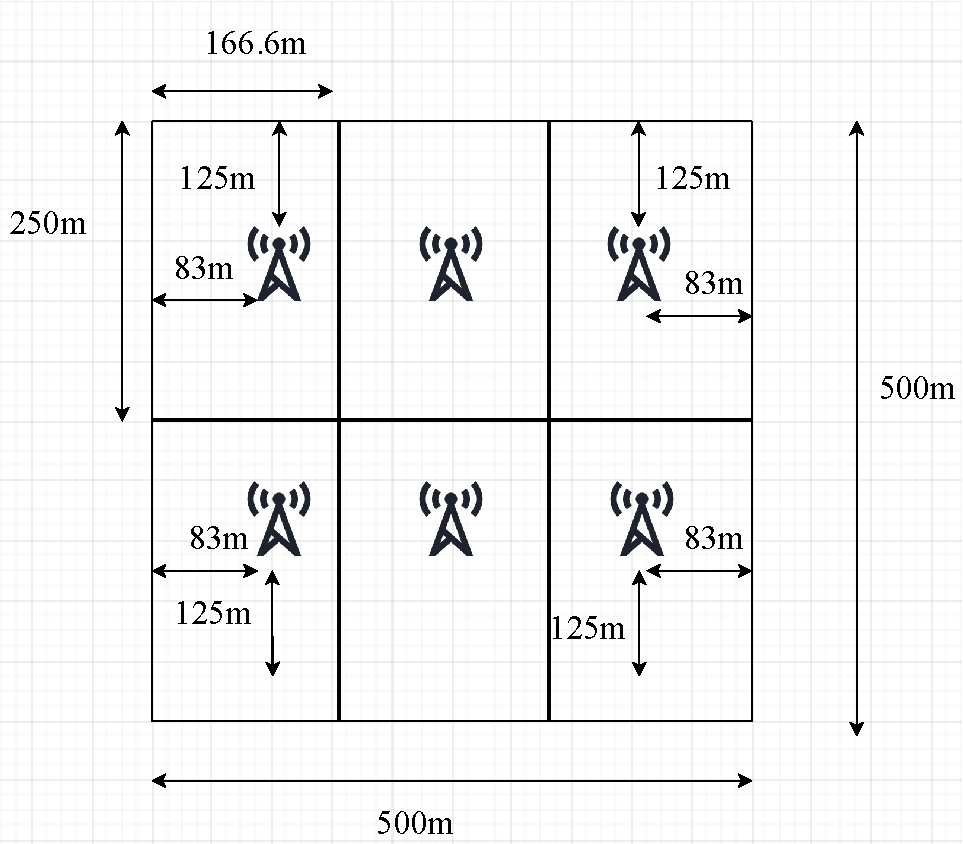
\includegraphics[scale = 0.47]{cell.pdf}
    %\includegraphics[max height=30cm,max width=9.5cm]{Drawing15.eps}
    %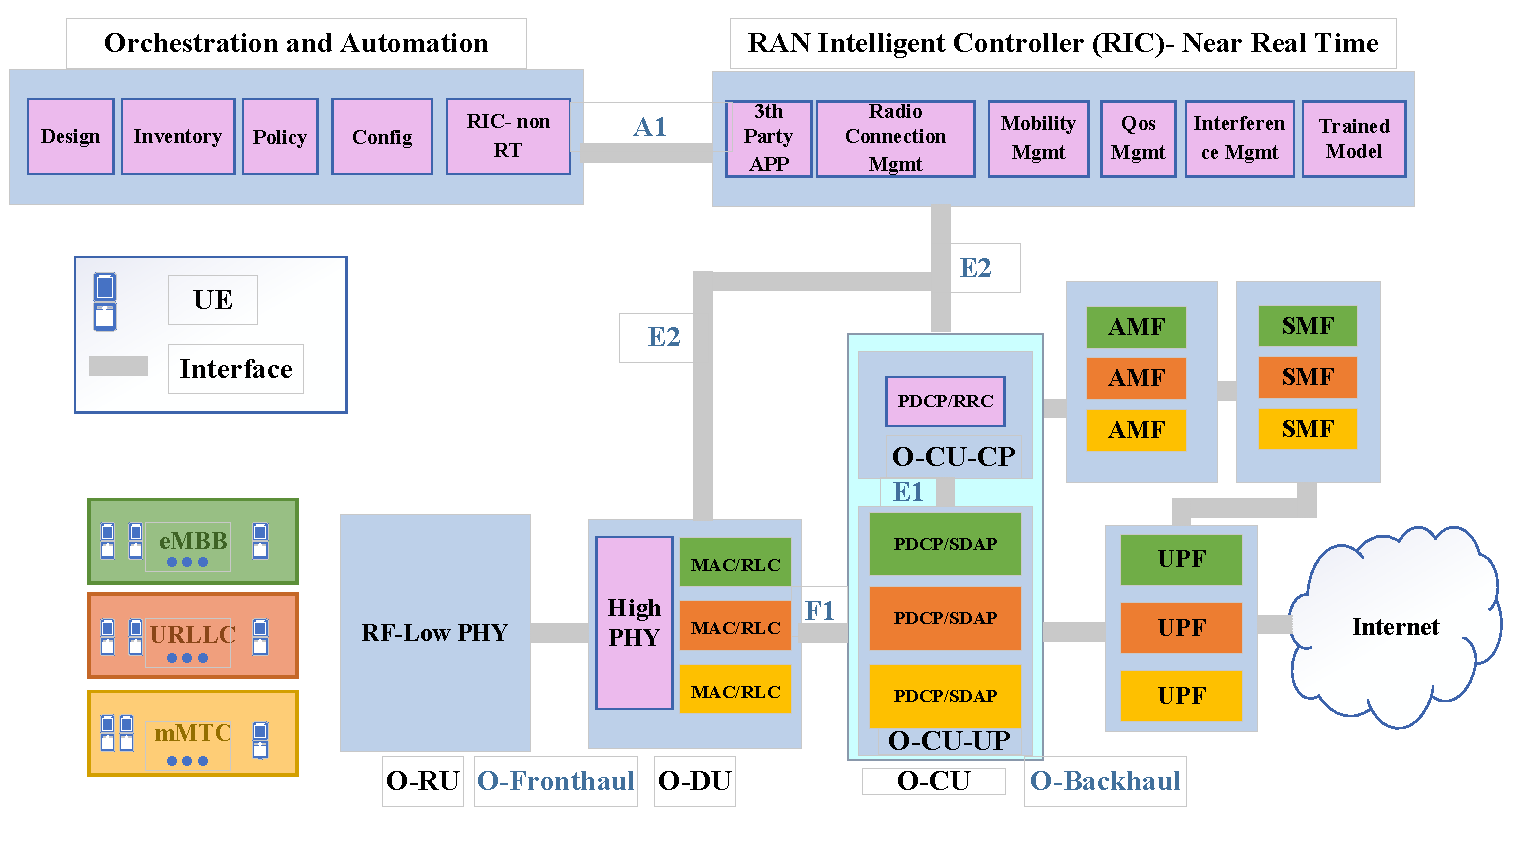
\includegraphics[width=\textwidth]{finalDraw.pdf}
  \caption{O-RU placement in a cell}
  \label{fig:cell}
\end{figure}
Here, the channel vector from the O-RU $r$ to the UE $i$ in service $s$ is set as $\bold{h}_{r,u(s,i)}^{k}=d_{r,u(s,i)}^{-\mathcal{L}} \Omega_{r,u(s,i)}^{k} $, where $d_{r,u(s,i)}^{-\mathcal{L}} $ is the distance between the O-RU $r$ and UE $i$ in service $s$ and $\mathcal{L} = 3.8$ is the path-loss exponent \cite{gholipoor2020cloud}.
Also, $\Omega_{r,u(s,i)}^{k}$ is the random variable that is generated by the Rayleigh distribution and it is the Rayleigh fading channel between the UE and O-RU.
We consider 25 PRBs are used in the network and the packet size is equal to 20 bytes.
The maximum number of VNF for each slice is 25 and the mean arrival data rate for the eMBB service is $\lambda  = 3Mbps$ and for the mMTC service and the URLLC  service is $\lambda  = 0.2Mbps$. 
Also, the quantization noise is assumed to be $10^{-13}$.
Moreover, we set $\mathfrak{h}_{u_{(s,i)}} = \eta_{u_{(s,i)}}/200$, $\mathfrak{m}_{r} = \zeta_r/10$
and $\mathfrak{q}^k_{r,u(s,i)} = P_{s}^{max}/100$. The other parameters of these simulations are depicted in Table \ref{table:1a}.
\begin{table}
 \caption {Simulation Parameters} \label{table:1a}
 \begin{center}
  \begin{tabular}{||c | c ||}
  \hline
Parameter & Value \\ [0.5ex]
  \hline\hline
  Noise power & -174dBm\\
  \hline
  Bandwidth & 180 KHz \\
  \hline
 Maximum transmit Power of each O-RU & 40dBm \\
  \hline
  Maximum delay for eMBB &  4msec \\
  \hline
    Maximum delay for URLLC &  1msec \\
  \hline
  Maximum delay for mMTC &  5msec \\
  \hline
  Maximum fronthaul capacity  & 46 bits/sec/Hz \\
   \hline
  Minimum data rate for eMBB &  20 bits/sec/Hz \\ 
  \hline
   Minimum data rate for URLLC and mMTC &  2 bits/sec/Hz \\ 
  \hline
   Maximum received power for mMTC &  20 dBm \\ [.5ex]   
  \hline
    Maximum received power for eMBB and URLLC &  33 dBm \\ [.5ex]   
  \hline
 \end{tabular}
 \end{center}
 \end{table}
 
Finding a feasible initial value is almost tricky. To overcome this challenge, we use a fast method that is discussed in \ref{fr}. If the fast method converges and has a feasible solution, so our algorithm (IABV) can be converged too.

Two different methods are used to compare with the performance of the proposed method (IABV) and show the optimality of our approach.
 The first one is a baseline scheme, which uses random PRB allocation. The association of O-RU is carried out based on distance. Also, the number of activated VNFs for each slice is fixed. The optimal power is obtained using the CVX of Matlab, which uses the successive convex approximation (SCA) method. The second one is similar to the FBDR algorithm proposed in \cite{lee2018dynamic}. In this method, PRB and power are dynamically allocated, and the number of VNFs is obtained from the simulation, and the UEs are associated with the O-RU based on the quality of their channels and the channel distance.
\subsection{Feasible Region}\label{fr}
Applying the correct initial point to make the system feasible is a significant step in our work.
During the simulations, it can be noted that sometimes the algorithm does not converge for some of the iterations with fixed initial values.
To solve this problem, we investigated the non-converging and converging simulation for models with fixed initial parameters (such as number of UEs, the threshold of power and rate,... ) and random channel gains of UEs.
By comparing convergent and non-convergent simulations, we experimentally found that in cases where convergence does not occur, there are UEs at the edge of the boundaries or far away from the O-RU and have a weak channel gain. One solution is to eliminate UEs who undermine system convergence.
For a large number of UEs with a fixed number of PRBs, the probability of having an infeasible solution increases due to a large number of UE interference.
Another solution is to remove the simulations in the mont-Carlo that do not converge.
In the simulation part, if more than half of the iterations have a feasible solution for the initial condition, the simulation can be displayed as a feasible model.
To remove non-converging simulations, we need to use a fast algorithm (FA) to check the convergence before
the proposed algorithm (IABV). 
If the conditions in \eqref{RConstr}, \eqref{pr11}, \eqref{c12-1} and \eqref{c12} are met in the fast algorithm (FA), the given algorithm will converge.
The FA algorithm is represented in Algorithm \ref{alg3}.

 \begin{algorithm}
\caption{Fast Algorithm (FA) to Check the Convergence}\label{alg3}
\begin{algorithmic}[1]
\State The number of UEs: $\mathfrak{N} = \sum_{s=1}^{S}\sum_{i=1}^{U_s}1$
\State The number of PRBs: $K$
\State the distance from the $r^{th}$ O-RU to the UE i in slice $s$: $d_{r,u(s,i)}$ 
\State Set count = 0 
\State Set $p_{r,u(s,i)}^{k} = 0 \quad \forall r,k,s,i$
\State Set $e_{r,u(s,i)}^{k} = 0 \quad \forall r,k,s,i$
\State Set $g_{u(s,i)}^{r} = 0 \quad \forall r,s,i$
\For{$s \gets 1$ to $S$} 
\For{$i \gets 1$ to $U_s$}
\State count = count +1  
\State $r^* = \argmin_r d_{r,u(s,i)} \quad \forall r$
\State $g_{u(s,i)} ^{r^*}=1$
\State temp =mod(count, K)            
\If {temp=0 }
\State $e_{r^*,u(s,i)}^{K} = 1 $
\State Set $p_{r^*,u(s,i)}^{K} = \min\{P_s^{\max}, P_r^{\max}/\mathfrak{N}\} $
\Else 
\State $e_{r^*,u(s,i)}^{\text{temp}} = 1 \quad \forall r$ 
\State Set $p_{r^*,u(s,i)}^{\text{temp}} = \min\{P_s^{\max}, P_r^{\max}/\mathfrak{N}\} $
\EndIf

\State \textbf{end if}
\EndFor
\State \textbf{end for}
\EndFor
\State \textbf{end for}
\end{algorithmic}
\end{algorithm}

The complexity order of this algorithm is $O(R\times \mathfrak{N})$ which is remarkably lower than the complexity order of the IABV method.
In the FA algorithm, the O-RU association is based on the distance of the UE to the O-RU. 
Each UE is associated with the nearest O-RU. Also, the power of each UE is set to be the minimum of the maximum power of each UE and the maximum power of each O-RU divided by the total number of UEs ($\min\{P_s^{\max}, P_r^{\max}/\mathfrak{N}\}$).
Moreover, the allocation of PRBs to UEs is based on dividing the number of UEs by the total number of PRBs.
If the number of UEs is more than the PRBs, each UE is given exactly one PRB without interference. Otherwise, the amount of interference will not be high but more than one UE will use same PRBs.
\subsection{Numerical Results}
In Fig. \ref{fig:1}, the aggregate throughput is demonstrated versus the different number of UEs in each service for these three methods. Suppose we have one service instance for each type of service, so we have three various services in this figure. Also, we have between 6 to 48 UEs in the system.
Here, we did not consider the priority. The figure presented that the proposed method, IABV, is $18.6\%$ higher throughput than the baseline scheme.
As the number of UEs increases in each service, the aggregated throughput initially increases. Still, due to the interference and the power constraint, it will be saturated from 12 UEs in each service.
\begin{figure}
  \centering 
    \includegraphics[scale = 0.47]{Arate_ue1.eps}
    %\includegraphics[max height=30cm,max width=9.5cm]{Drawing15.eps}
    %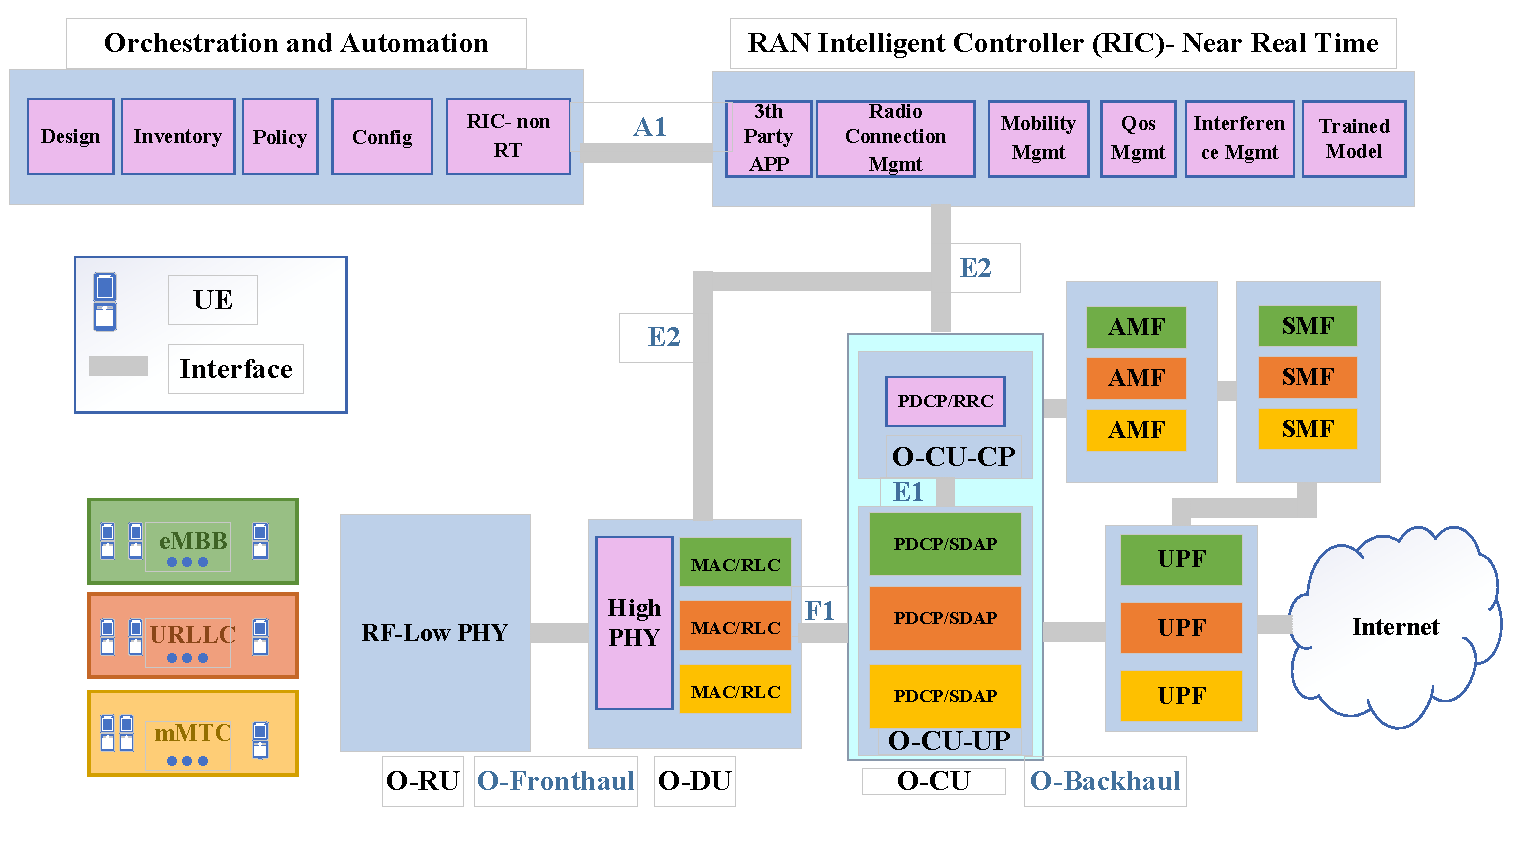
\includegraphics[width=\textwidth]{finalDraw.pdf}
  \caption{Aggregate throughput vs. number of UEs for each service in the presence of three services}
  \label{fig:1}
\end{figure}
%Assume we have two type of services (URLLC and mMTC). In figure \ref{fig:2} and \ref{fig:3}, the aggregate throughput (by considering the priority factor 
%($\sum_s \sum_i \delta_s \bar{R}_{{u(s,i)}}$)) is depicted for two services URLLC and mMTC. Here we consider 4 UEs in each service. The other parameter is shown in table \ref{table:1a}.
%The figure \ref{fig:2}, presented that by increasing the priority factor for URLLC, more resources is allocated to this service and the aggregate throughput of this service is increased and vice verse.
%\begin{figure}
%  \centering 
%    \includegraphics[scale = 0.4]{mmtcURLLC.eps}
%    %\includegraphics[max height=30cm,max width=9.5cm]{Drawing15.eps}
%    %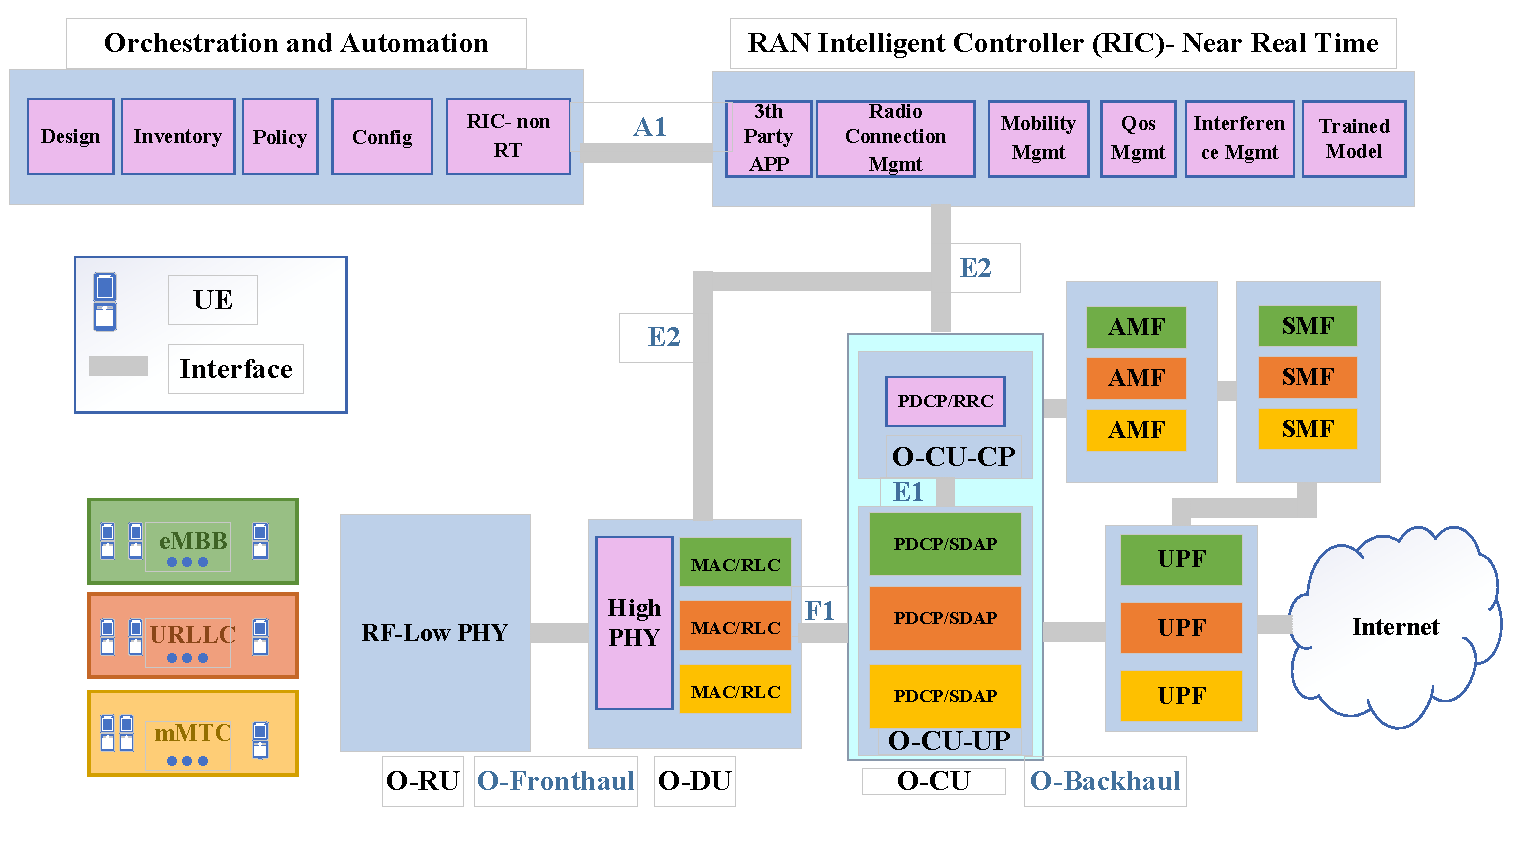
\includegraphics[width=\textwidth]{finalDraw.pdf}
%  \caption{Aggregate Throughput for mMTC and URLLC vs. Priority of URLLC }
%  \label{fig:2}
%\end{figure}
%In figure \ref{fig:3}, the total sum rate of URLLC and mMTC is shown vs. priority of URLLC. It is shown that the proposed method is much better than the baseline scheme. 
%\begin{figure}
%  \centering 
%    \includegraphics[scale = 0.4]{sumRatePri.eps}
%    %\includegraphics[max height=30cm,max width=9.5cm]{Drawing15.eps}
%    %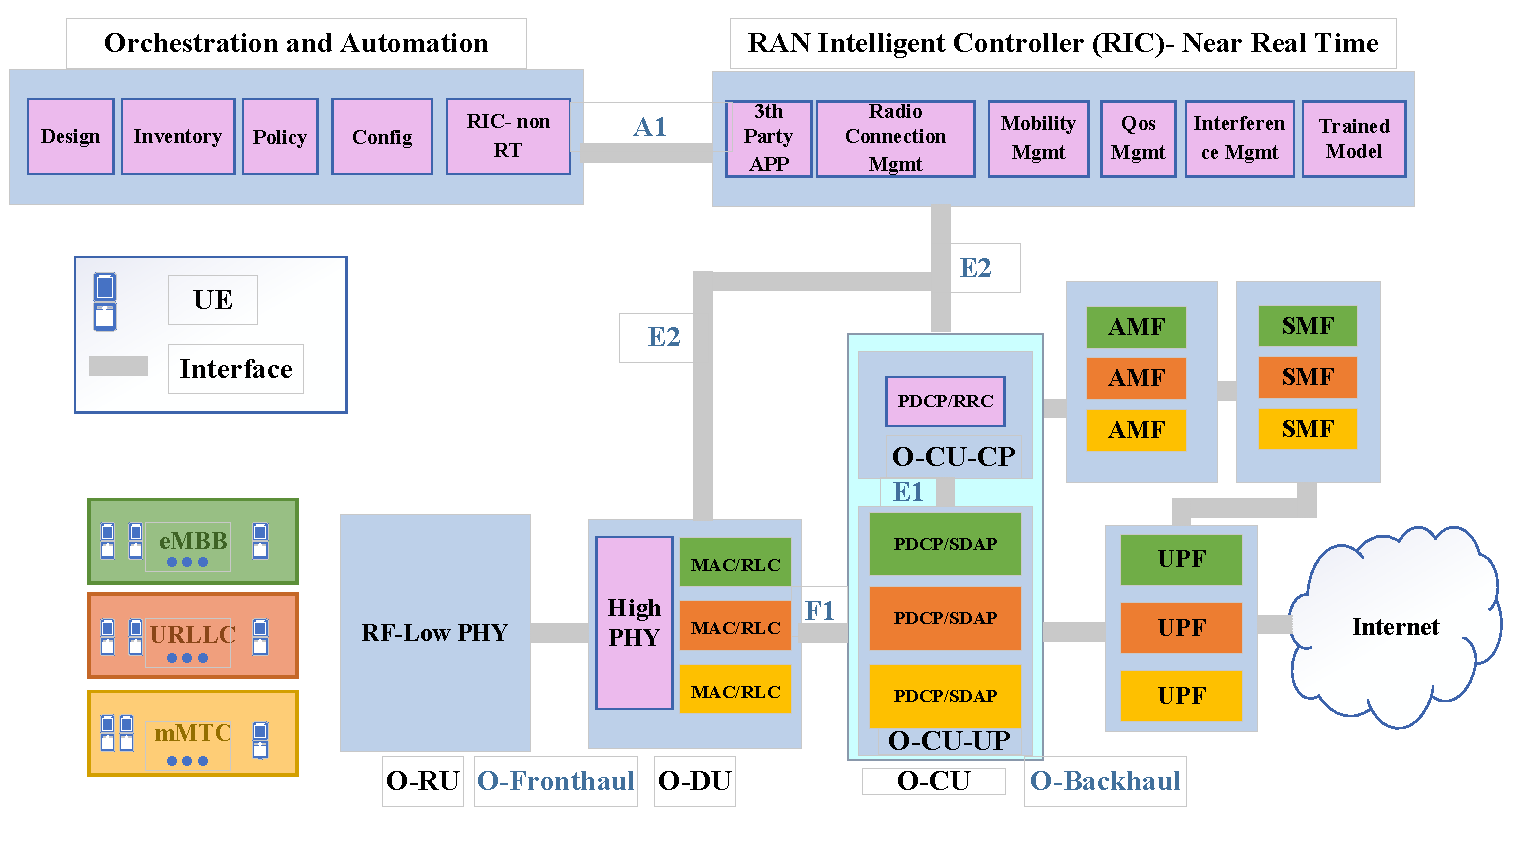
\includegraphics[width=\textwidth]{finalDraw.pdf}
%  \caption{Aggregate Throughput of all services vs. Priority of URLLC}
%  \label{fig:3}
%\end{figure}

Figure \ref{fig:4} depicts the number of activated VNFs for five different mean service times of one URLLC service vs. the mean arrival time for 12 UEs. This figure presents that as the mean arrival rate increases, the number of activated VNF increases. Moreover, the number of activated VNFs decreases when the mean service rate increases.


\begin{figure}
  \centering 
    \includegraphics[scale = 0.47]{vnfNum1.eps}
    %\includegraphics[max height=30cm,max width=9.5cm]{Drawing15.eps}
    %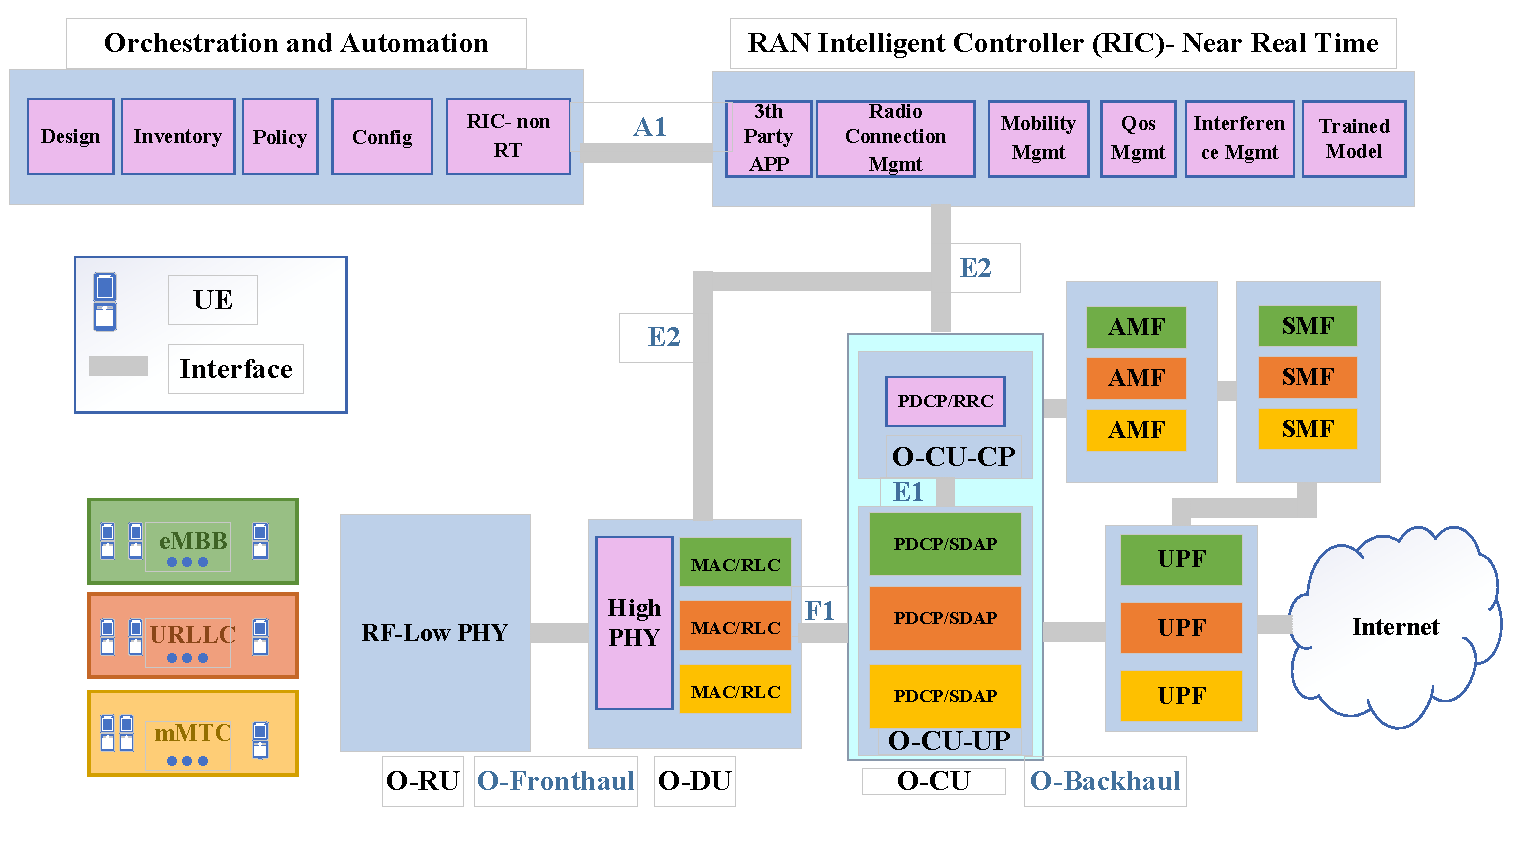
\includegraphics[width=\textwidth]{finalDraw.pdf}
  \caption{Number of activated VNF in each Service vs. Mean Arrival Rate(Mbps)}
  \label{fig:4}
\end{figure}

In figure \ref{fig:5}, the aggregate throughput is depicted vs. the maximum power of UE for three different instances of eMBB service using proposed method (IABV), FBDR and the baseline scheme. Here, we suppose that we have 12 UEs in each service.  We assume that these three services require 5bits/sec/Hz, 10bits/sec/Hz, and 15bits/sec/Hz.
In addition, We suppose that each O-RU can transmit three times of the maximum power of the UEs. As you can see in the figure, increasing the maximum power increases the aggregate throughput. Moreover, the proposed method (IABV), gives higher aggregate rates in compared to the FBDR and the baseline scheme.  

\begin{figure}
  \centering 
    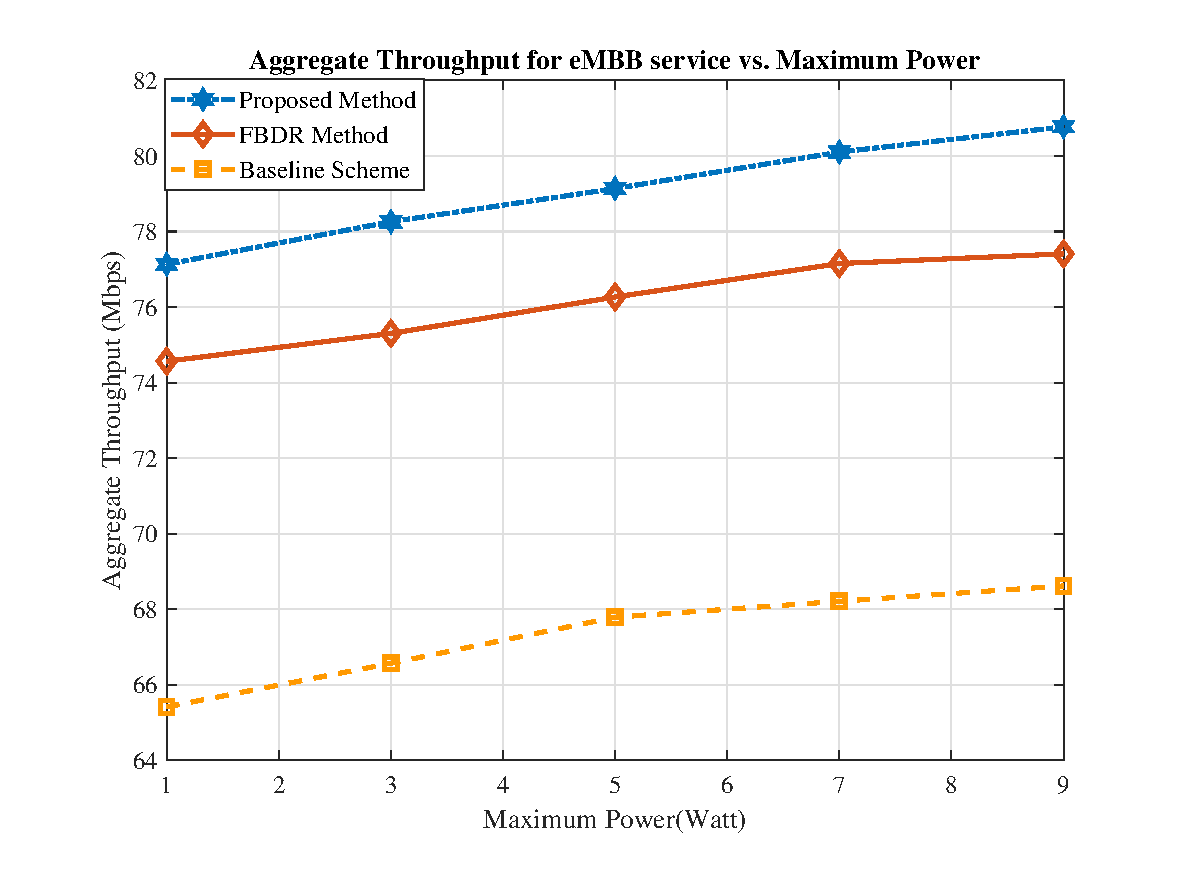
\includegraphics[scale = 0.47]{RatePower1.eps}
    %\includegraphics[max height=30cm,max width=9.5cm]{Drawing15.eps}
    %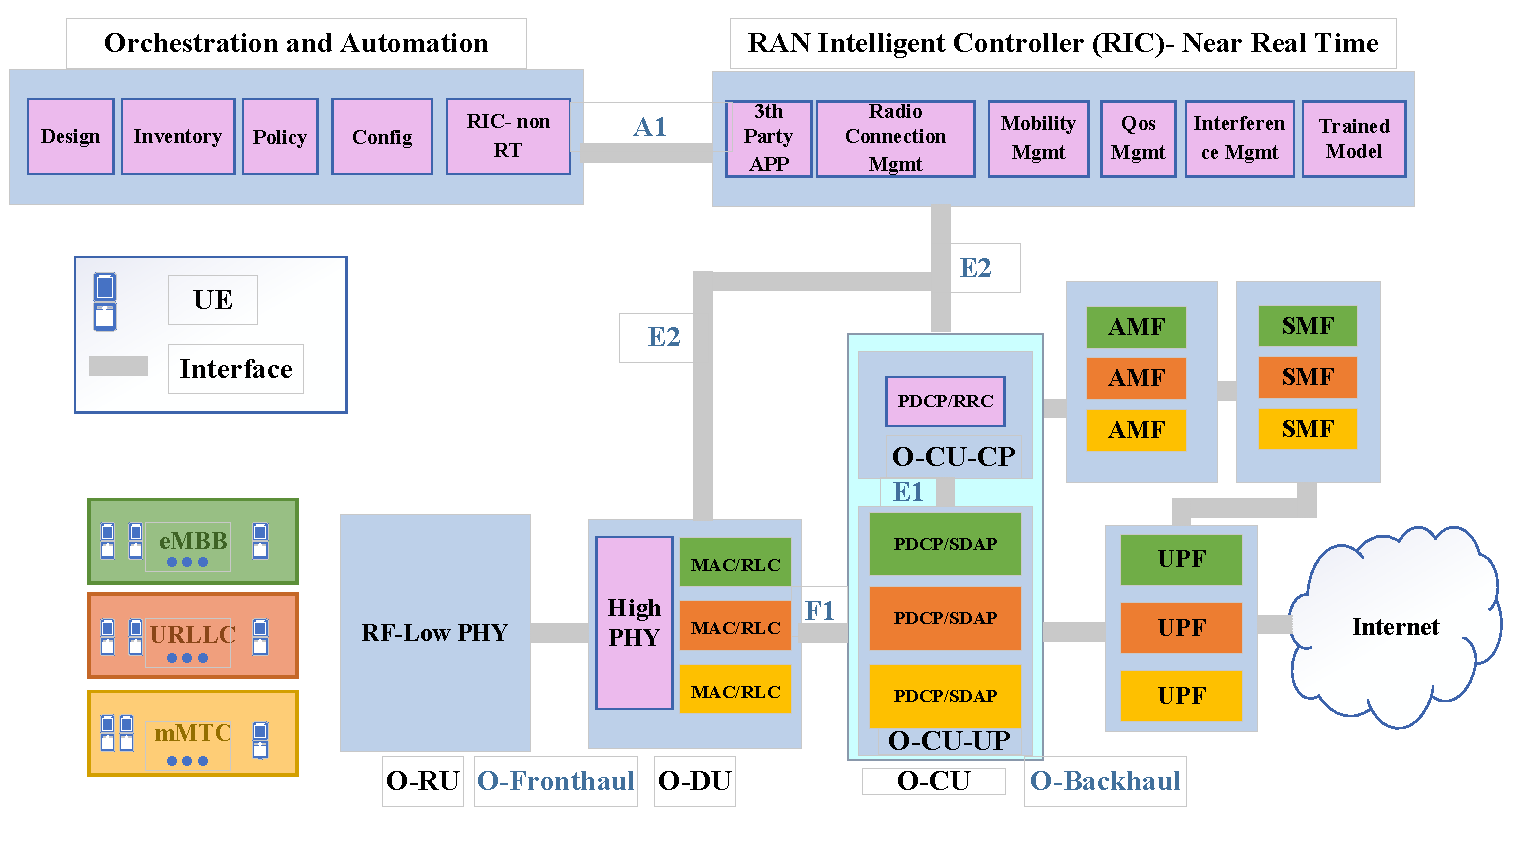
\includegraphics[width=\textwidth]{finalDraw.pdf}
  \caption{Aggregate Throughput for eMBB vs. Maximum Transmit power for various number of UEs }
  \label{fig:5}
\end{figure}

Figure \ref{fig:6} illustrates the mean total delay of a UE in a URLLC service regarding the mean arrival rate of the UE and the number of UEs in the service for the proposed method (IABV).
It is shown that the delay is an ascending function of the mean arrival rate (when the mean service time is fixed) and the number of UEs in the service. In this figure, we assume that the maximum number of VNF for each slice is 50 and the maximum delay of each UE in a URLLC service is $0.5ms$. Also, the maximum number of PRB is considered to be 50. 
 Moreover, we can see that the mean delay of a URLLC service 
does not reach the maximum threshold of the delay.
%Moreover, we can see that the mean delay of a URLLC service increases almost linearly with the mean arrival rate of the packet transmission. 
\begin{figure}
  \centering 
    \includegraphics[scale = 0.47]{delay_new.eps}
    %\includegraphics[max height=30cm,max width=9.5cm]{Drawing15.eps}
    %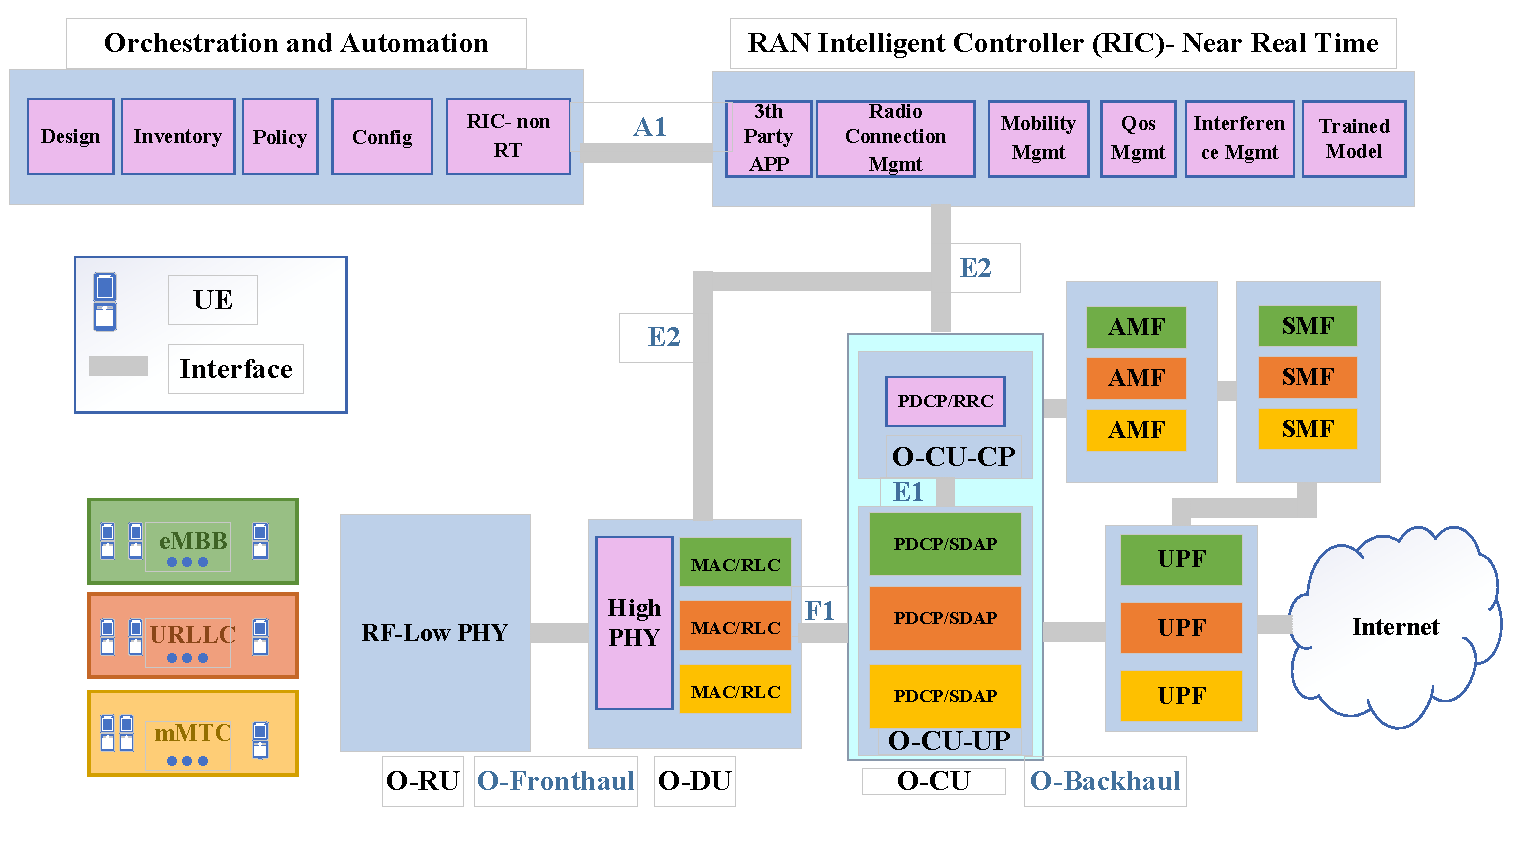
\includegraphics[width=\textwidth]{finalDraw.pdf}
  \caption{Mean Total Delay of a URLLC Service vs. the Mean Arrival Rate of a UE in the Service for various number of UEs}
  \label{fig:6}
\end{figure}
Figure \ref{fig:7} is the same as figure \ref{fig:6} that presented the mean total delay of a UE in a URLLC service regarding the mean arrival rate of the UE for 20 UEs using three different methods. As you can see, the proposed method (IABV) outperforms the other scenarios.

\begin{figure}
  \centering 
    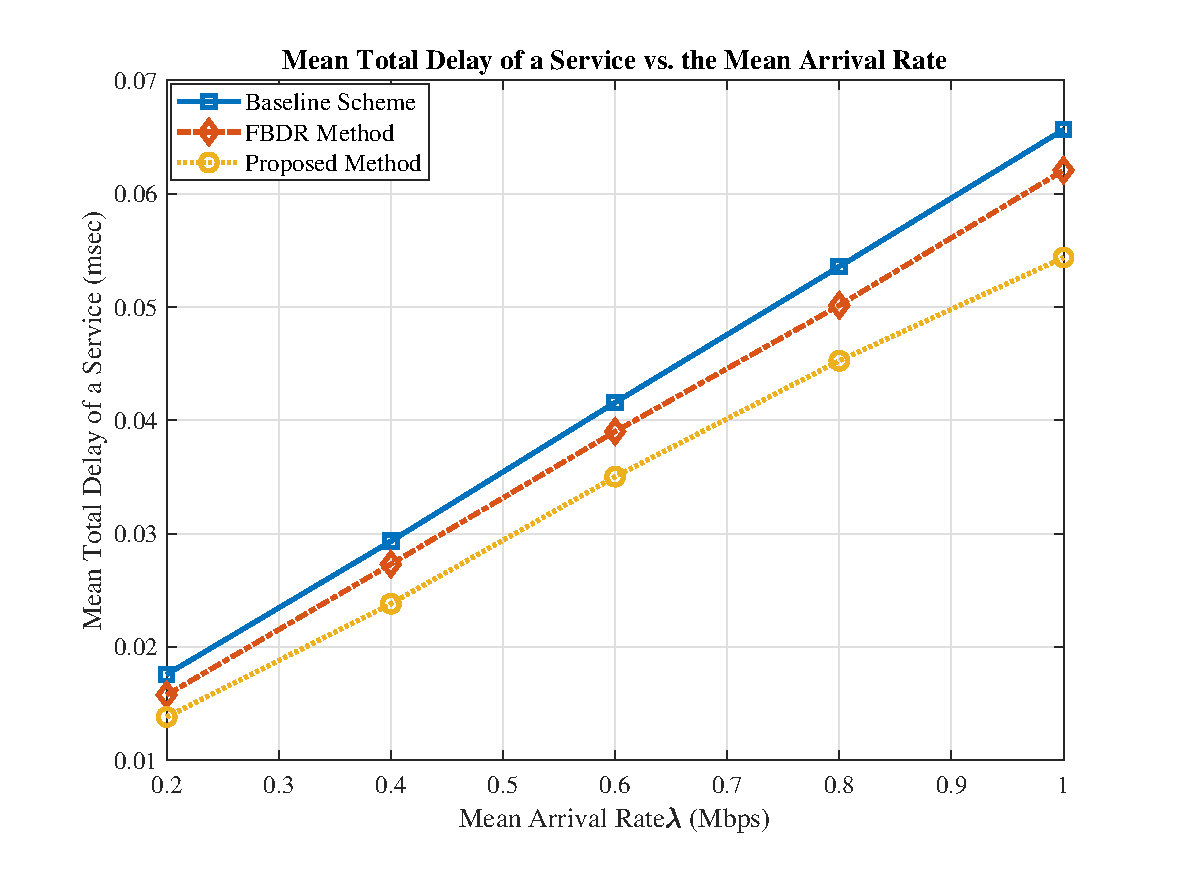
\includegraphics[scale = 0.47]{delay1_new.eps}
    %\includegraphics[max height=30cm,max width=9.5cm]{Drawing15.eps}
    %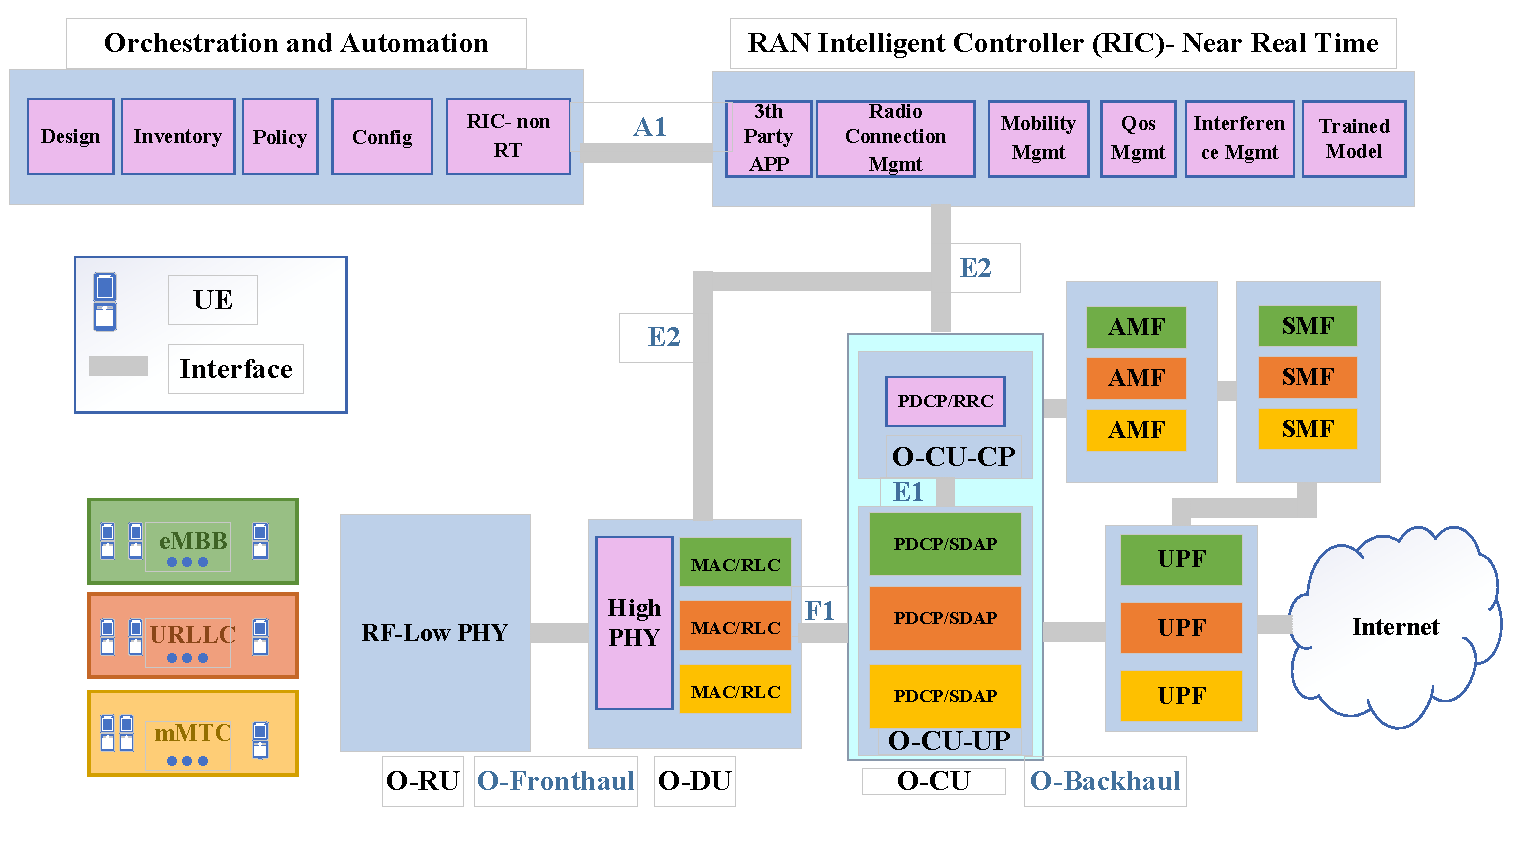
\includegraphics[width=\textwidth]{finalDraw.pdf}
  \caption{Mean Total Delay of a URLLC Service vs. the Mean Arrival Rate of a UE in the Service for different methods}
  \label{fig:7}
\end{figure}

Figure \ref{fig:8}, represents the aggregate throughput concerning the number of UEs in each service and the maximum power for three different mMTC service instances. mMTC service includes a large number of UEs with low data rates and low power. 
Assume each UE in each mMTC service instance requires 0.1 bits/sec/Hz data rate and is not sensitive to the end-to-end delay. Also, suppose the fronthaul link and the number of VNFs have no restrictions.
%Moreover, to make the simulation feasible, we assume that the number of PRBs is as large as the system has low interference.
%so we suppose there is a fixed  PRB allocation in the simulation that each UE is allocated to one PRB. There is no PRB with more than one UE allocation.
The figure depicts that by increasing the number of UEs in each instance of the service, the aggregate throughput increases. 
Also, by increasing the maximum power of each UE in each instance of mMTC service, the aggregate throughput rises too.
\begin{figure}
  %\centering 
    \includegraphics[scale = 0.4]{AmmTCpower.eps}
    %\includegraphics[max height=30cm,max width=9.5cm]{Drawing15.eps}
    %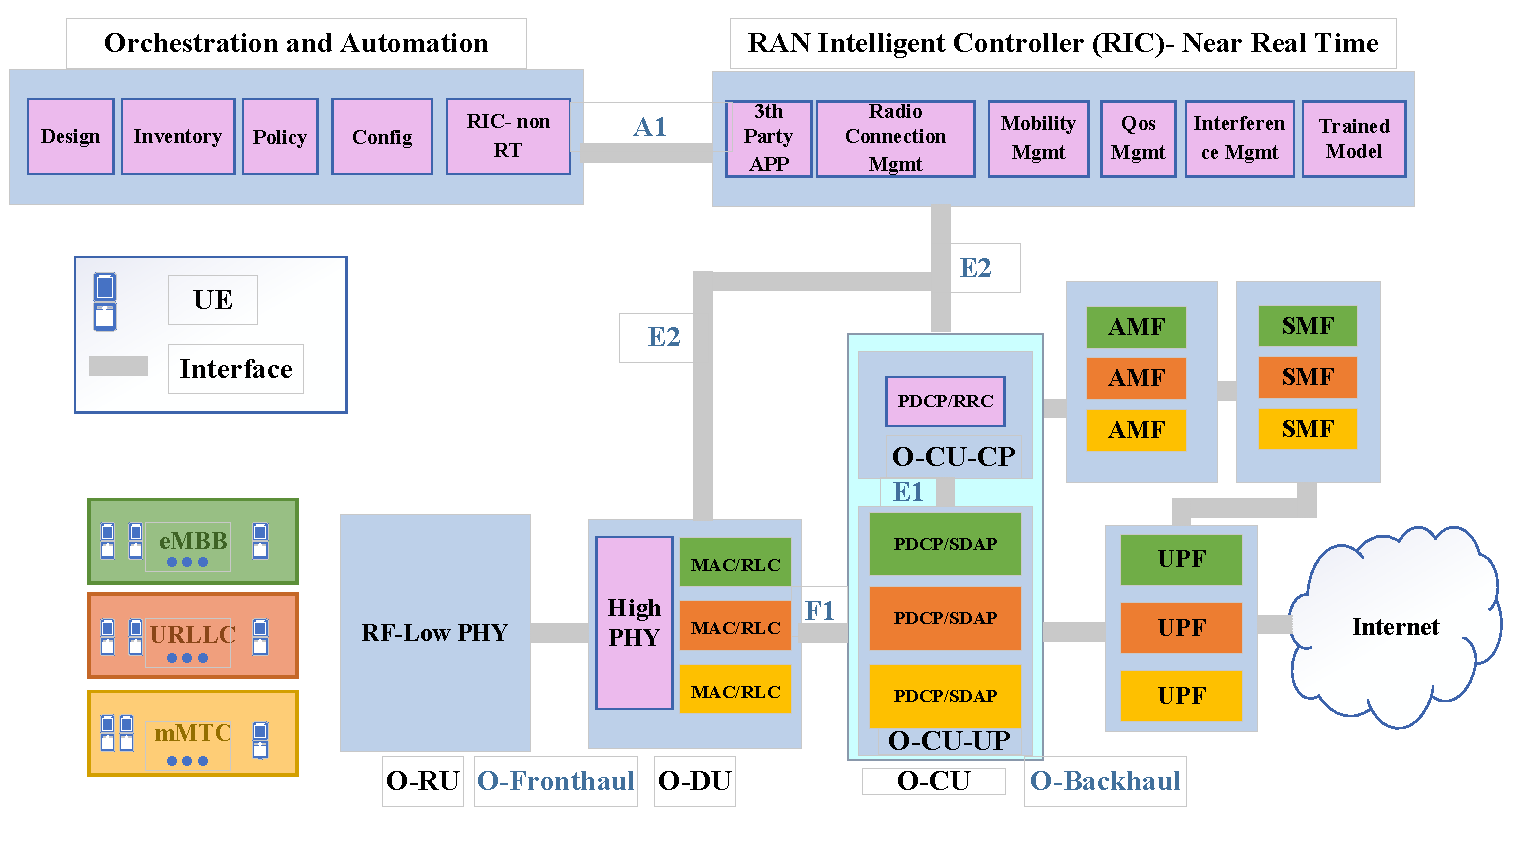
\includegraphics[width=\textwidth]{finalDraw.pdf}
  \caption{Aggregate Throughput for mMTC services vs. Number of UEs in each Service for three different mMTC service instances}
  \label{fig:8}
\end{figure}

Assume we have two types of eMBB service instances. In figure \ref{fig:9}, the aggregate throughput (by considering the priority factor $\delta_s$) is depicted for two eMBB service instances. Here we consider 4 UEs in each service. We assume that the the fronthaul link and the end-to-end delay have no restrictions.
The figure \ref{fig:9} presented that by increasing the priority factor for one service instance, more resources are allocated to this service instance, and the aggregate throughput of this service is increased and vice versa. Also, we can realize from this figure that the aggregate throughput has the most significant value at the same priority.
\begin{figure}
  \centering 
    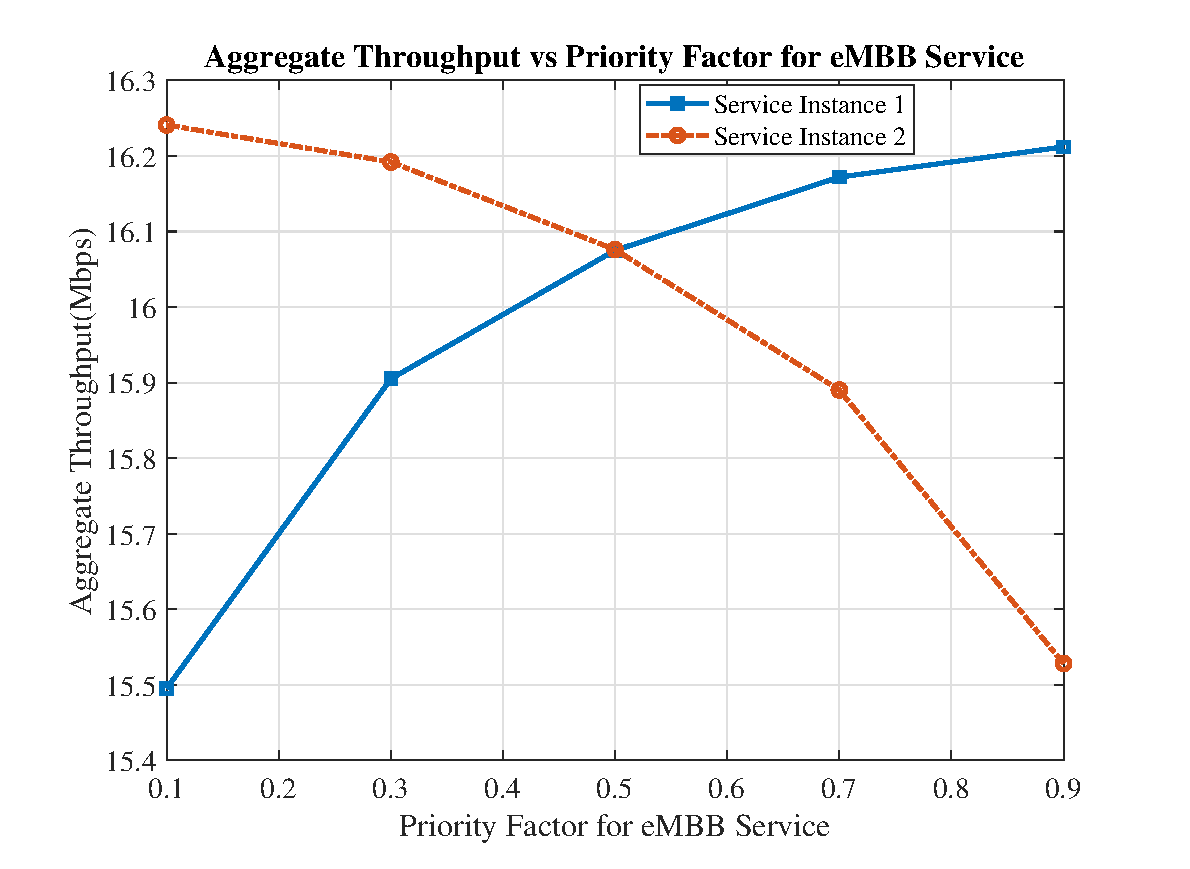
\includegraphics[scale = 0.4]{priorityLast.eps}
    %\includegraphics[max height=30cm,max width=9.5cm]{Drawing15.eps}
    %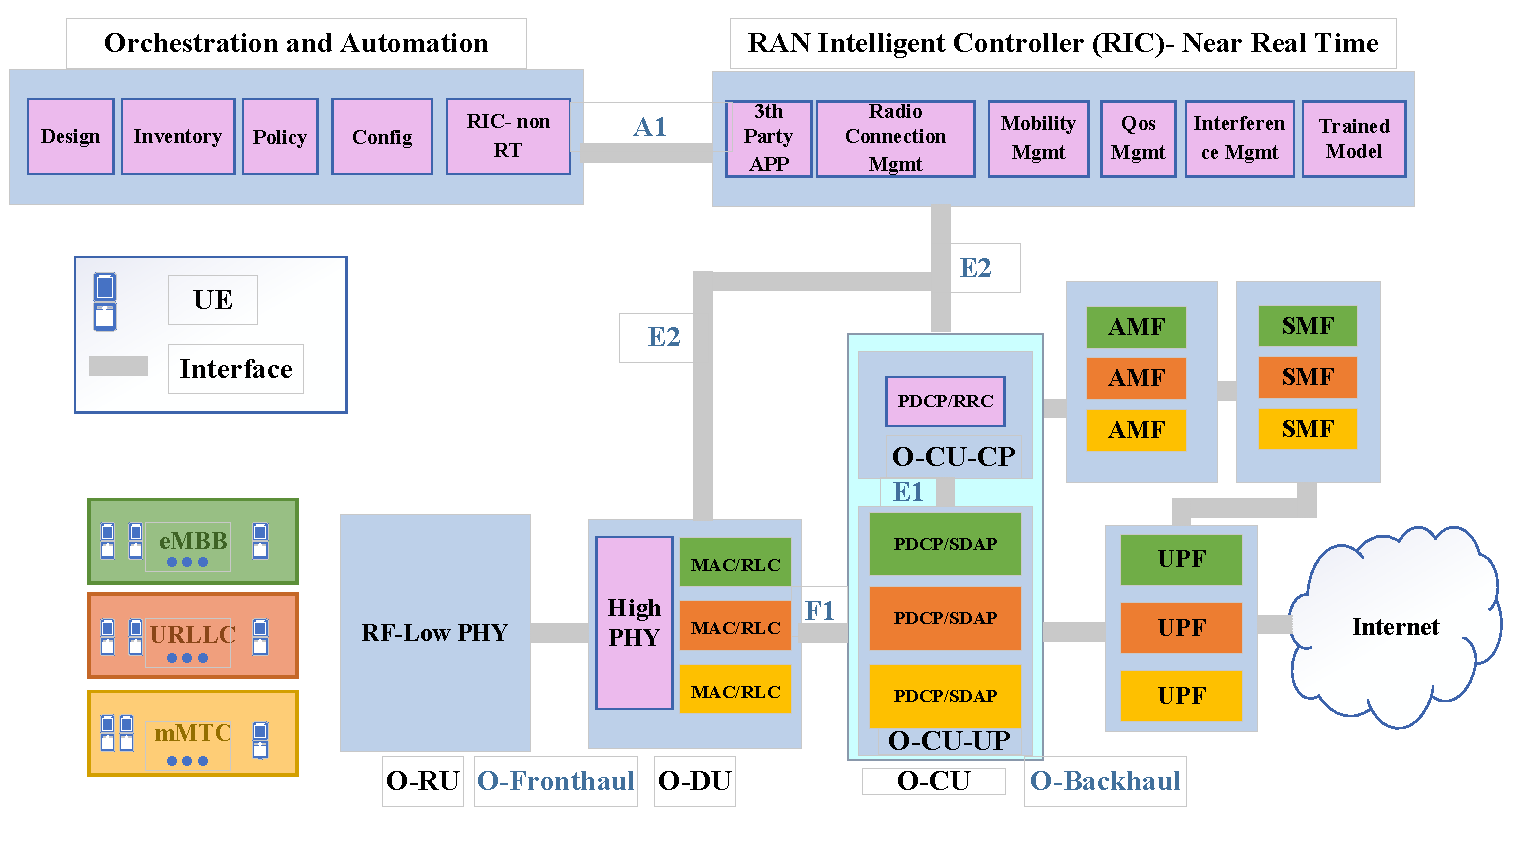
\includegraphics[width=\textwidth]{finalDraw.pdf}
  \caption{Aggregate Throughput for two eMBB service instances vs. Priority of the first service instance }
  \label{fig:9}
\end{figure}
%
%In the figure \ref{fig:10}, the aggregate throughput is presented vs. the number of UEs for one service in a system by considering two different cloud restrictions and fronthaul restrictions.
%In the graph of cloud restriction, we have the restrictions in O-DU and O-CU.
%In the graph of fronthaul restriction, we have the restrictions in O-RU.
%In the O-RU restriction graph, we assume that the fronhaul link is set to be 47 bits/sec/Hz (the variance of quantization noise is $10^{-13}$) , and the maximum power of each O-RU is 40 dBm. Also, the maximum power of each UE is set to be 35 dBm. Moreover, the minimum data rate for each UE in this service is 6 bits/sec/Hz. In this graph, we assume that there is less restriction in the end-to-end delay (50 ms) and the VNF resources (the system has 100 reserved VNF).
%In the graph of cloud restriction, we assume that there is no restriction on the fronthaul link.
%The limitation on the power is less than the graph of fronthaul limitation, and it is set to be 45 dBm on the power of each O-RU, and the maximum power of each UE is 40 dBm.
%The minimum data rate for each UE in this service is 10 bits/sec/Hz. 
%The end-to-end delay for each UE is 4ms and the mean arrival rate is 2Mbps. 
%and the mean service rate is 10Mbps.
%In this figure, the consequence of cloud limitation and fronthaul limitation is depicted.
%As the number of UEs increases, the aggregate throughput rises linearly, and the graph of cloud restriction increases more than the other graph of fronthaul limitation. 

%\begin{figure}
%  \centering 
%    \includegraphics[scale = 0.4]{AcloudVsFronthaul.eps}
%    %\includegraphics[max height=30cm,max width=9.5cm]{Drawing15.eps}
%    %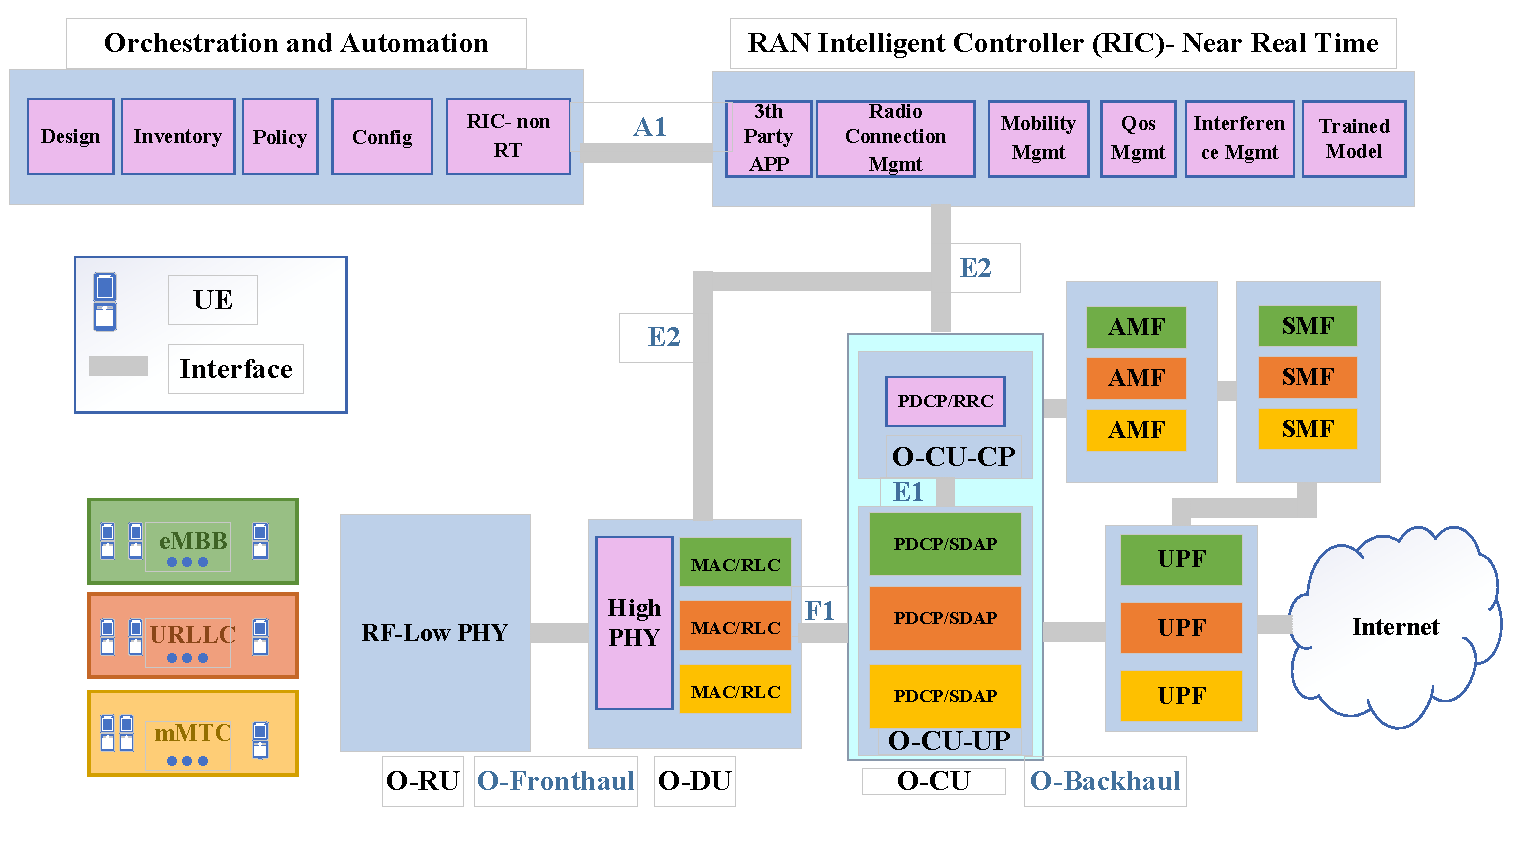
\includegraphics[width=\textwidth]{finalDraw.pdf}
%  \caption{Aggregate Throughput vs. Number of UEs in a Service}
%  \label{fig:10}
%\end{figure}
In figure \ref{fig:11}, the aggregate throughput is shown according to the number of iteration (outer loop) of the
proposed algorithm (IABV) for different numbers of UEs for one service. In this figure, the convergence of the IABV method is illustrated. The minimum data rate for each UE is assumed to be 2 Mbps.
After four iterations, IABV converges to the fixed value.



\begin{figure}
  \centering 
    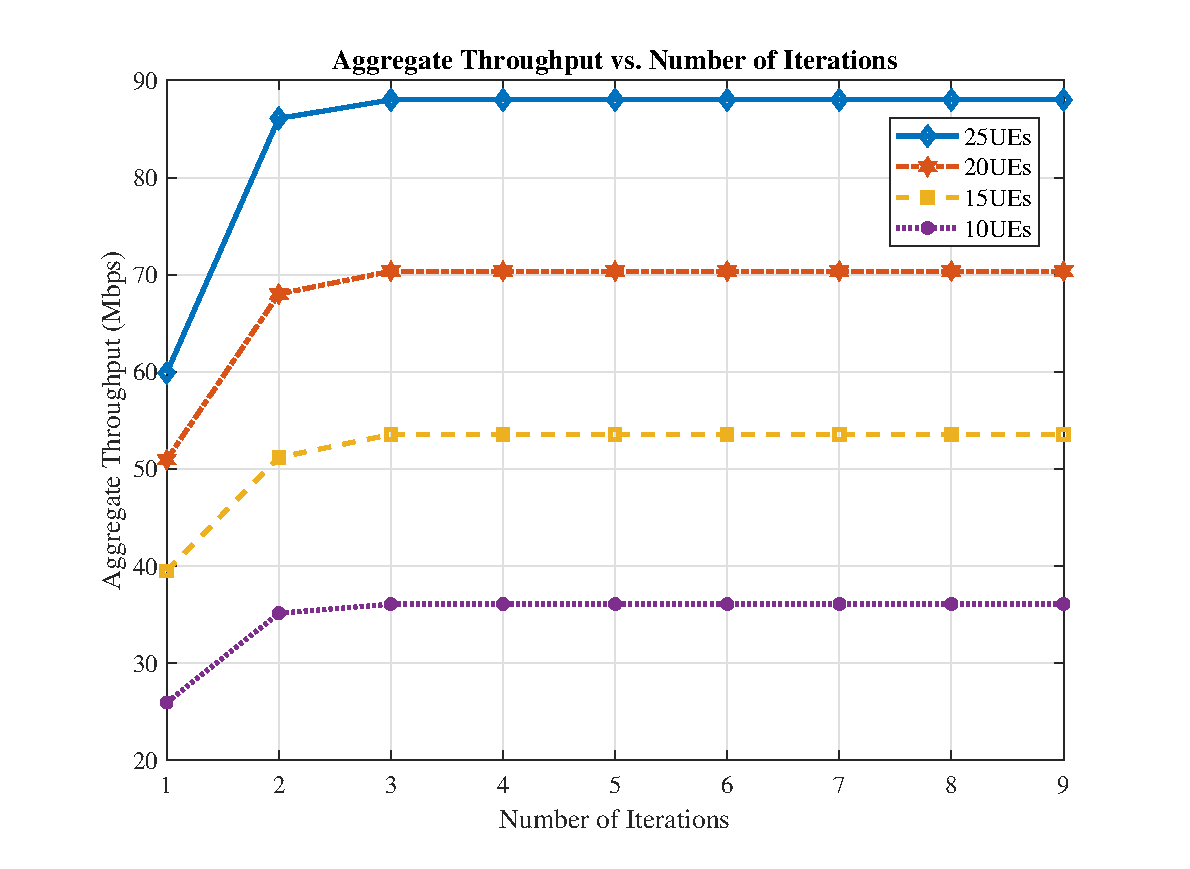
\includegraphics[scale = 0.4]{iter.eps}
    %\includegraphics[max height=30cm,max width=9.5cm]{Drawing15.eps}
    %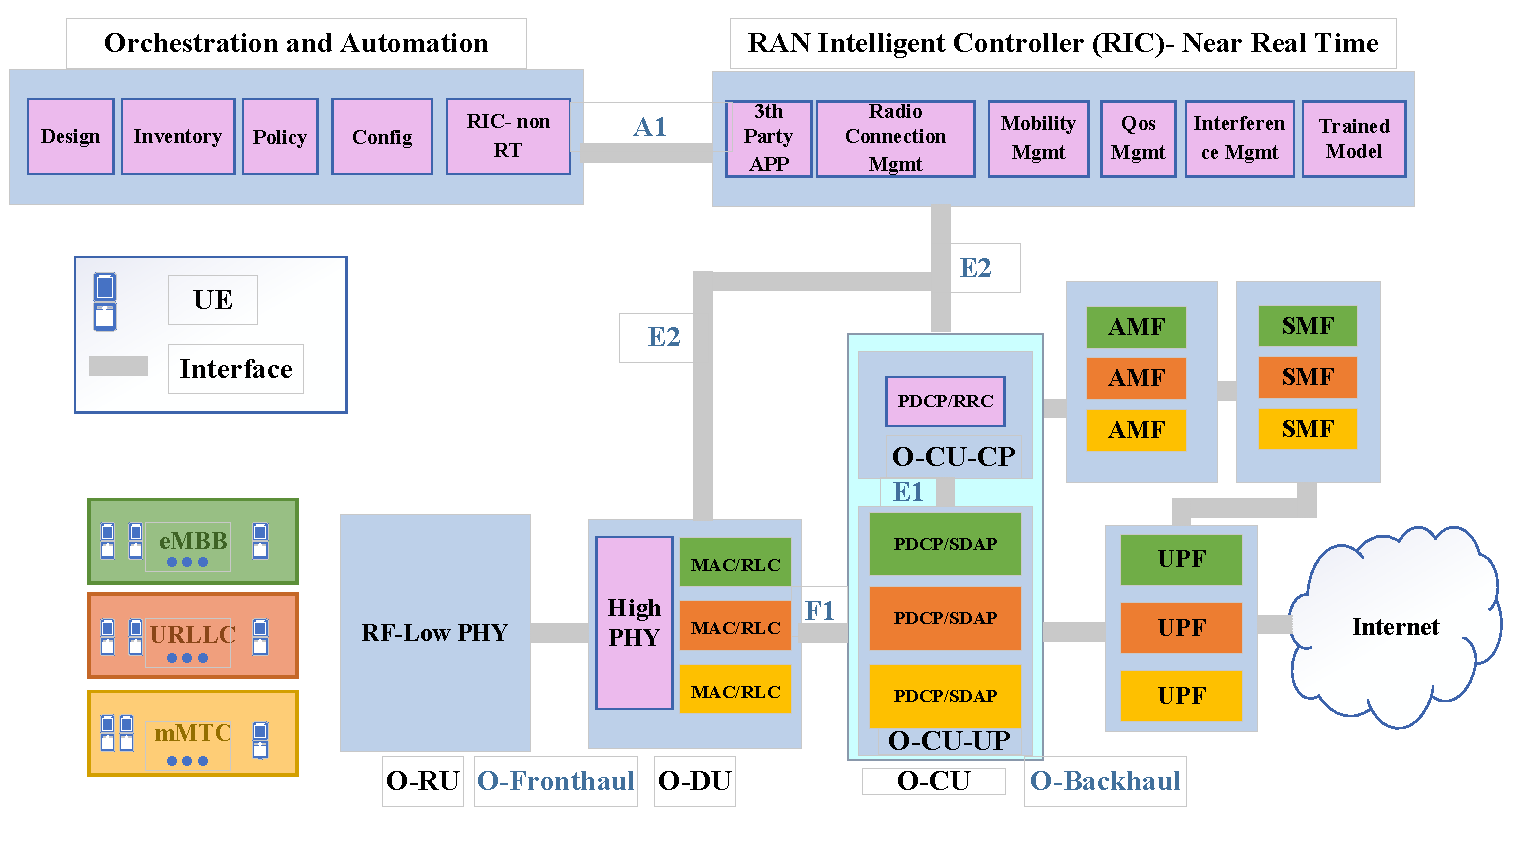
\includegraphics[width=\textwidth]{finalDraw.pdf}
  \caption{Aggregate Throughput vs. Number of Iterations}
  \label{fig:11}
\end{figure}

%\subsection{Summary of Simulation Results}
In figure \ref{fig:12}, the aggregate throughput is shown according to the number of UEs for two different methods, namely the
proposed algorithm (IABV) and the optimal method for URLLC service for the low interference.
The minimum data rate is 5bits/sec/Hz for each UE and the maximum delay is $0.1$ms.
Also the mean arrival rate is set to be $0.2$Mbps and the mean service rate is $0.5$Mbps.
The other parameters are depicted in table \ref{table:1a}.
The optimal approach is obtained from the two-step joint exhaustive search and using CVX. 
In each iteration in the first step, the PRB allocation and O-RU association are obtained from brute force, and in the second step, we use CVX to get optimal power.
Our solution is close to the optimal value in a small number of UEs.
\begin{figure}
  \centering 
    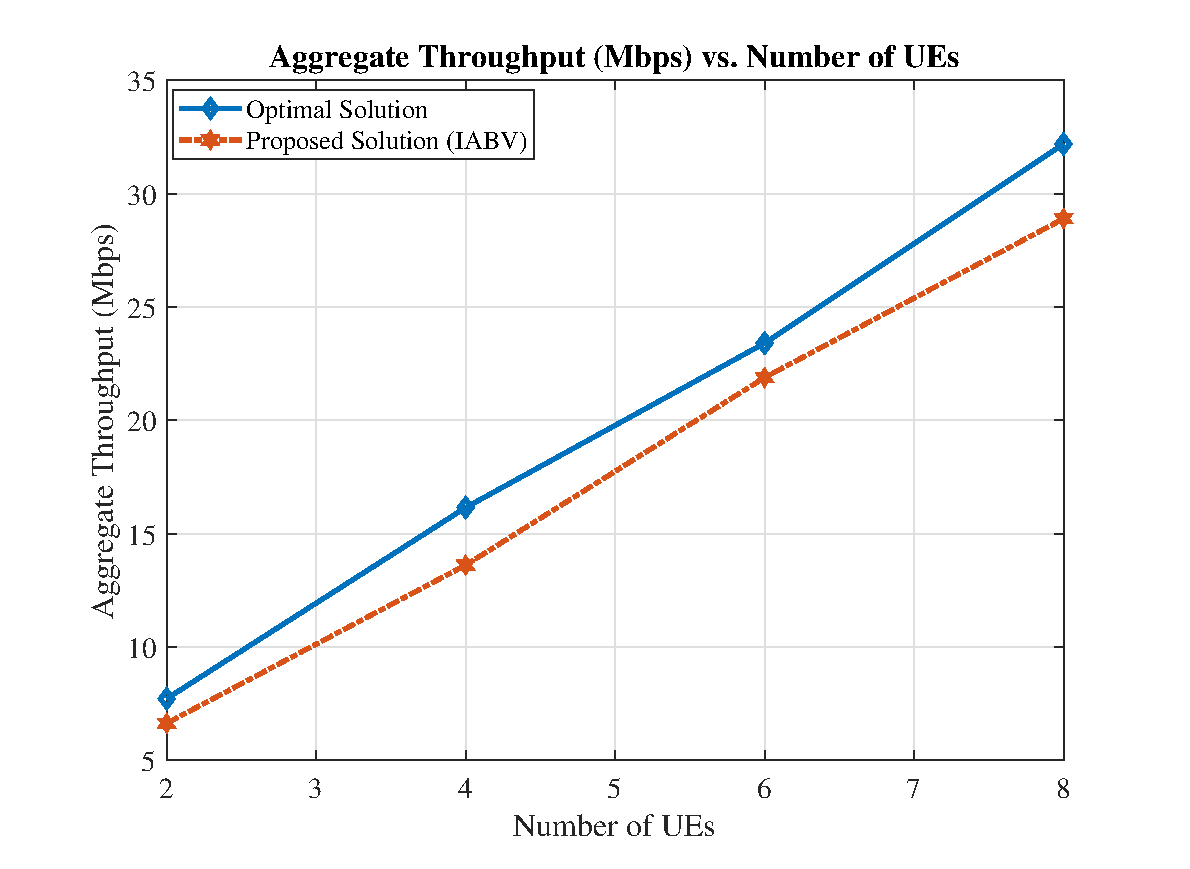
\includegraphics[scale = 0.4]{optimal1.eps}
    %\includegraphics[max height=30cm,max width=9.5cm]{Drawing15.eps}
    %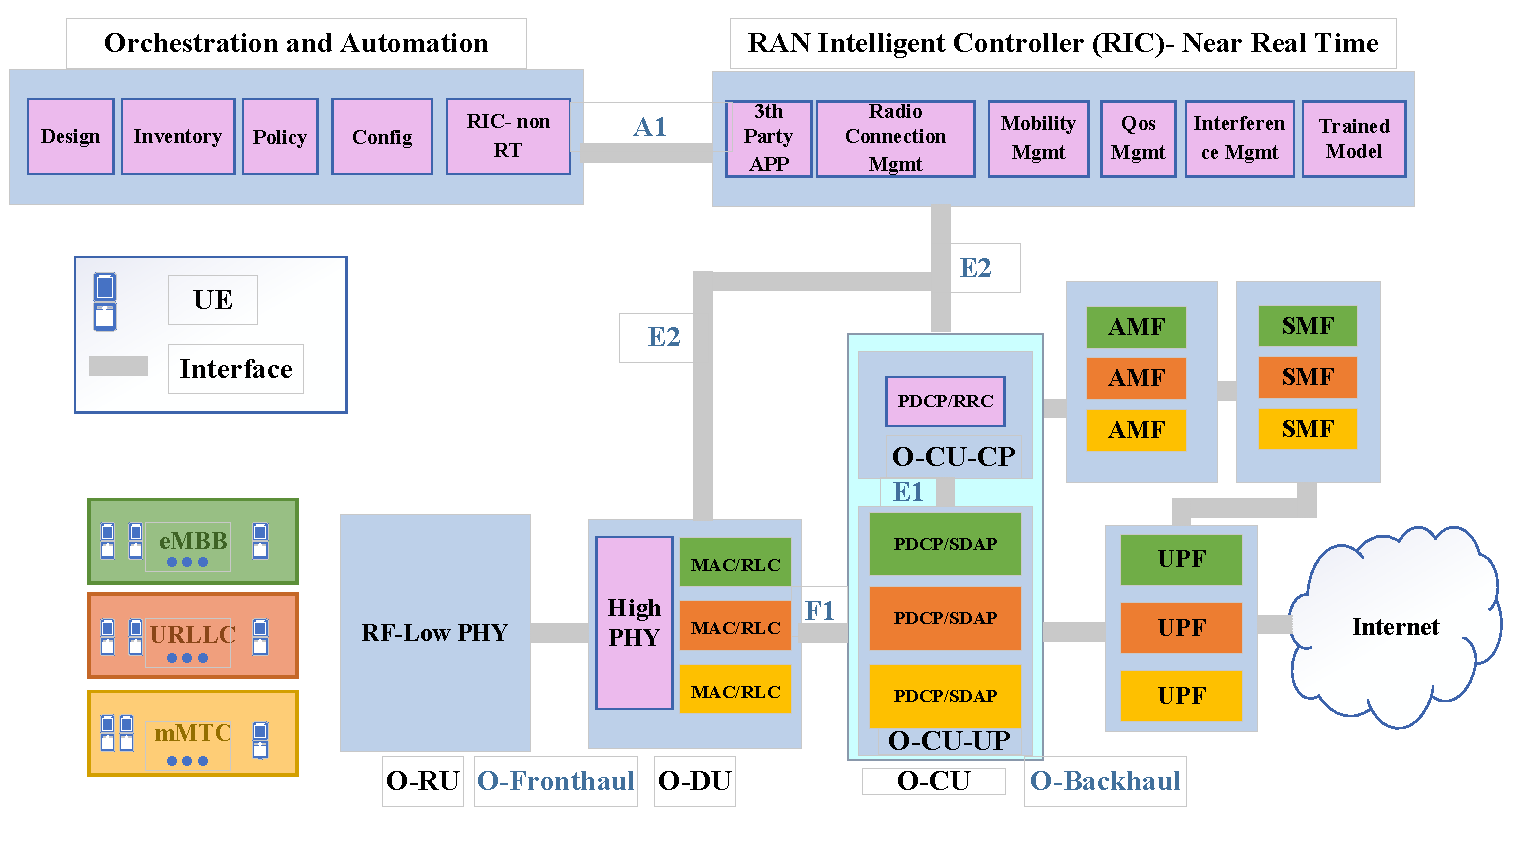
\includegraphics[width=\textwidth]{finalDraw.pdf}
  \caption{Aggregate Throughput vs. Number of UEs }
  \label{fig:12}
\end{figure}

In figure \ref{fig:13}, the aggregate throughput is depicted vs. the maximum interference for two different maximum power thresholds of O-RU. We suppose that the maximum power threshold of UEs is one-third of the maximum power of O-RU.
%The minimum data bit rate is assumed to be 0.2Mbps for each UE.
Here we assume that with the increase of every ten dBm of interference power, it is assumed that ten users have been added to the system. In -105 dBm, we have 5 UEs, and at the end, we have 55 UEs in the system.
Since the amount of interference in the system is entered as a fixed value,
the allocation of PRBs is not considered.
The higher maximum power threshold leads to a greater aggregate throughput. 
The aggregate throughput first increases with the number of UEs and at the same time the amount of the maximum interference, then it becomes almost fixed and finally decreases so much. When the aggregate throughput decreases, the maximum interference is so high that it takes the system out of feasibility.
%The aggregate throughput rises with the increases of UEs and the maximum interference and then remains almost constant.

\begin{figure}
  \centering 
    \includegraphics[scale = 0.4]{interF_new.eps}
    %\includegraphics[max height=30cm,max width=9.5cm]{Drawing15.eps}
    %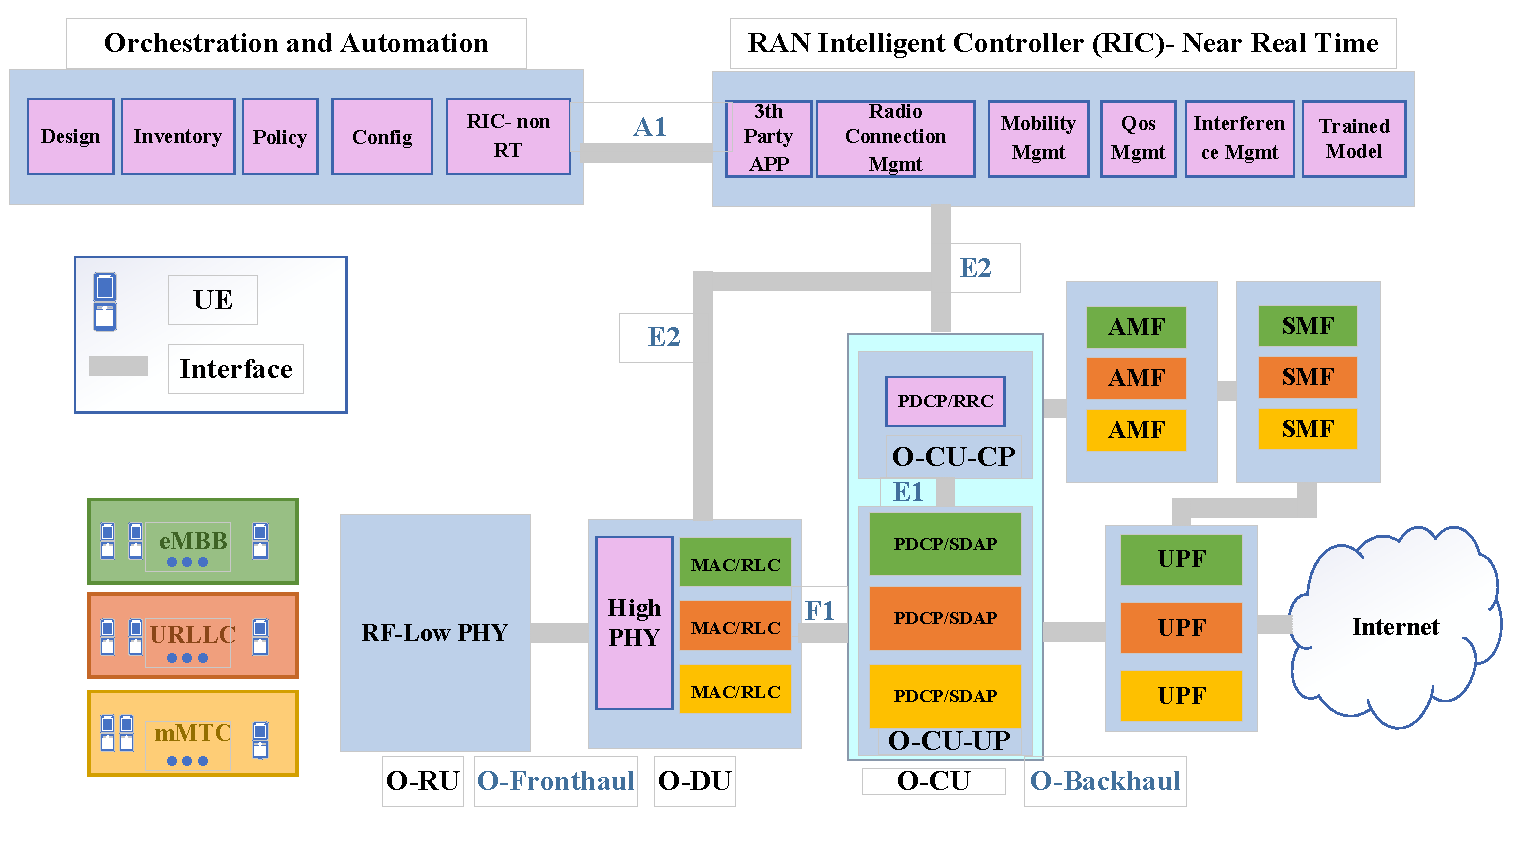
\includegraphics[width=\textwidth]{finalDraw.pdf}
  \caption{Aggregate Throughput vs. Maximum Interference }
  \label{fig:13}
\end{figure}

In figure \ref{fig:14}, the aggregate throughput is shown versus
the different number of UEs for an eMBB service with low interference for the IABV and FA methods in the feasible region.
The minimum data rate for each UE is 1Mb/s/Hz.
The maximum power for each O-RU is 34dBm, and the maximum power for each UE is 30dBm. We assume that the system is not sensitive to fronhaul capacity and end-to-end delay and has enough VNF resources.
By increasing the number of UEs, the aggregate throughput raises.
And we can see that the IABV method is better than the FA method. 

\begin{figure}
  \centering 
    \includegraphics[scale = 0.4]{FA.eps}
    %\includegraphics[max height=30cm,max width=9.5cm]{Drawing15.eps}
    %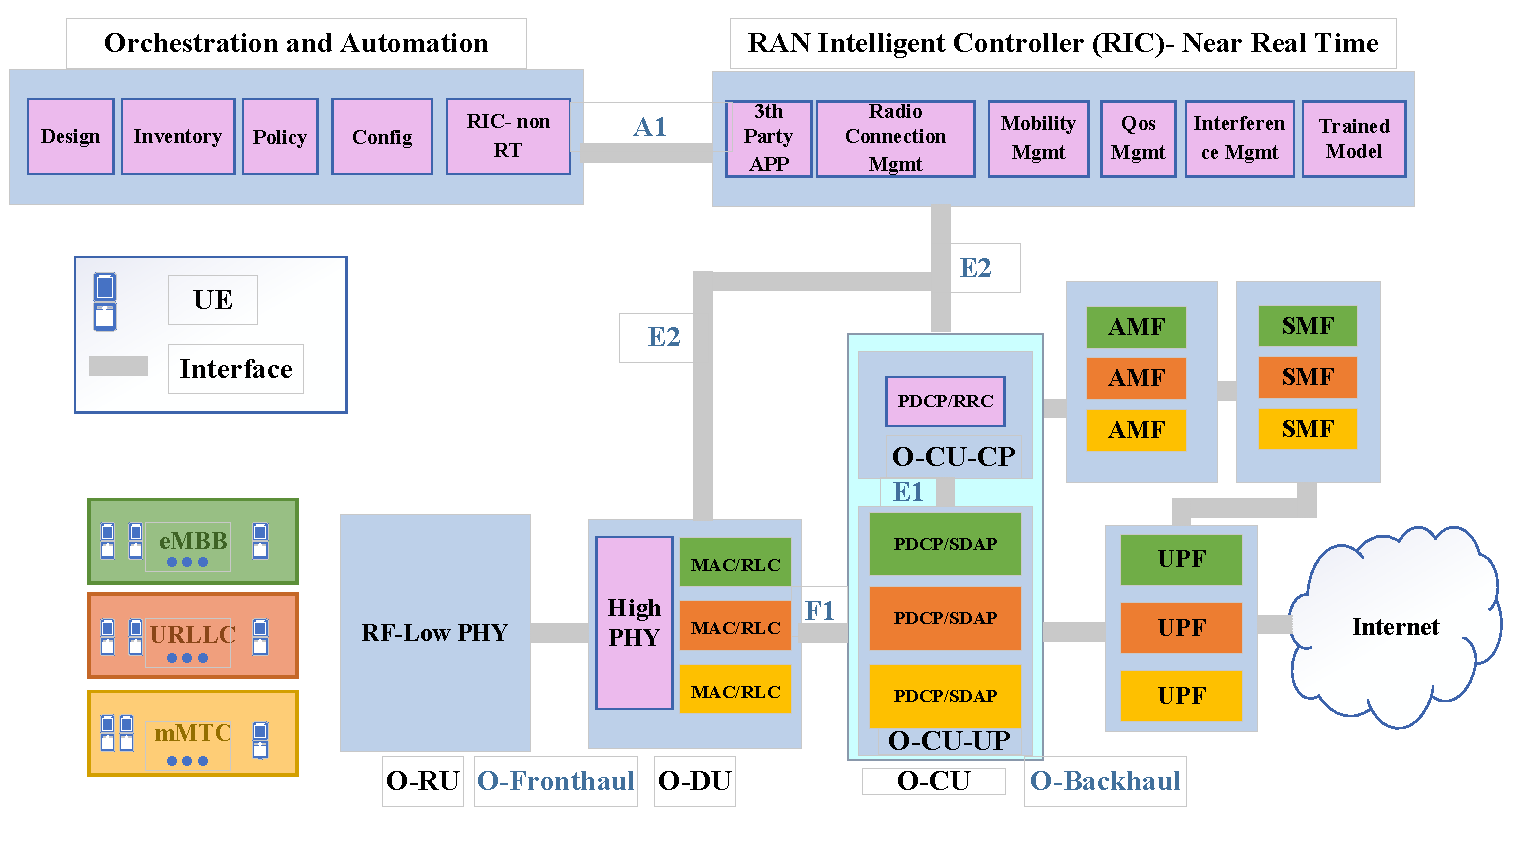
\includegraphics[width=\textwidth]{finalDraw.pdf}
  \caption{Aggregate Throughput vs. the Number of UEs }
  \label{fig:14}
\end{figure}

\section{Conclusion}\label{conc}
In this  paper, we modeled the downlink of the O-RAN system using network slicing for different 5G services, i.e., eMBB, mMTC, and URLLC.
The isolation of various services, i.e., eMBB, mMTC, and URLLC in the O-DU, the O-CU, and the UPF, is accomplished.
Also, the paper aims to obtain the number of activated VNFs in each service, RU association, power, and PRB allocation to maximize the aggregate throughput. The limited fronthaul capacity and the mean end-to-end delay for each service are considered. 
The problem is mixed-integer non-linear programming that is solved by a two-step iterative algorithm.
In the first step, we reformulated the problem to achieve the number of activated VNFs as a function of data rate. Then, we obtained PRB association and power allocation using the Lagrangian method.
In the second step, the O-RU association is carried out.
The performance of our proposed method (i.e., IABV) is compared with the baseline scheme and FBDR in \cite{lee2018dynamic}. 
In addition, the feasible region is discussed, and the FA algorithm is introduced to check the feasibility of the initial values.
Also, we assume distinct scenarios for each service, i.e., eMBB, mMTC, and, URLLC based on their requirement QoS.
Simulation results show that the proposed method (i.e., IABV) achieves $18.6\%$ higher data rate than the baseline scheme.
Moreover, simulation results illustrate more minor delays for the proposed method (IABV) than FBDR and the baseline scheme.


\bibliographystyle{IEEEtran} 
\bibliography{ref}
\end{document} 